\documentclass[twoside]{book}

% Packages required by doxygen
\usepackage{fixltx2e}
\usepackage{calc}
\usepackage{doxygen}
\usepackage[export]{adjustbox} % also loads graphicx
\usepackage{graphicx}
\usepackage[utf8]{inputenc}
\usepackage{makeidx}
\usepackage{multicol}
\usepackage{multirow}
\PassOptionsToPackage{warn}{textcomp}
\usepackage{textcomp}
\usepackage[nointegrals]{wasysym}
\usepackage[table]{xcolor}

% Font selection
\usepackage[T1]{fontenc}
\usepackage[scaled=.90]{helvet}
\usepackage{courier}
\usepackage{amssymb}
\usepackage{sectsty}
\renewcommand{\familydefault}{\sfdefault}
\allsectionsfont{%
  \fontseries{bc}\selectfont%
  \color{darkgray}%
}
\renewcommand{\DoxyLabelFont}{%
  \fontseries{bc}\selectfont%
  \color{darkgray}%
}
\newcommand{\+}{\discretionary{\mbox{\scriptsize$\hookleftarrow$}}{}{}}

% Page & text layout
\usepackage{geometry}
\geometry{%
  a4paper,%
  top=2.5cm,%
  bottom=2.5cm,%
  left=2.5cm,%
  right=2.5cm%
}
\tolerance=750
\hfuzz=15pt
\hbadness=750
\setlength{\emergencystretch}{15pt}
\setlength{\parindent}{0cm}
\setlength{\parskip}{0.2cm}
\makeatletter
\renewcommand{\paragraph}{%
  \@startsection{paragraph}{4}{0ex}{-1.0ex}{1.0ex}{%
    \normalfont\normalsize\bfseries\SS@parafont%
  }%
}
\renewcommand{\subparagraph}{%
  \@startsection{subparagraph}{5}{0ex}{-1.0ex}{1.0ex}{%
    \normalfont\normalsize\bfseries\SS@subparafont%
  }%
}
\makeatother

% Headers & footers
\usepackage{fancyhdr}
\pagestyle{fancyplain}
\fancyhead[LE]{\fancyplain{}{\bfseries\thepage}}
\fancyhead[CE]{\fancyplain{}{}}
\fancyhead[RE]{\fancyplain{}{\bfseries\leftmark}}
\fancyhead[LO]{\fancyplain{}{\bfseries\rightmark}}
\fancyhead[CO]{\fancyplain{}{}}
\fancyhead[RO]{\fancyplain{}{\bfseries\thepage}}
\fancyfoot[LE]{\fancyplain{}{}}
\fancyfoot[CE]{\fancyplain{}{}}
\fancyfoot[RE]{\fancyplain{}{\bfseries\scriptsize Generated on Mon Sep 28 2015 17\+:22\+:32 for My Project by Doxygen }}
\fancyfoot[LO]{\fancyplain{}{\bfseries\scriptsize Generated on Mon Sep 28 2015 17\+:22\+:32 for My Project by Doxygen }}
\fancyfoot[CO]{\fancyplain{}{}}
\fancyfoot[RO]{\fancyplain{}{}}
\renewcommand{\footrulewidth}{0.4pt}
\renewcommand{\chaptermark}[1]{%
  \markboth{#1}{}%
}
\renewcommand{\sectionmark}[1]{%
  \markright{\thesection\ #1}%
}

% Indices & bibliography
\usepackage{natbib}
\usepackage[titles]{tocloft}
\setcounter{tocdepth}{3}
\setcounter{secnumdepth}{5}
\makeindex

% Hyperlinks (required, but should be loaded last)
\usepackage{ifpdf}
\ifpdf
  \usepackage[pdftex,pagebackref=true]{hyperref}
\else
  \usepackage[ps2pdf,pagebackref=true]{hyperref}
\fi
\hypersetup{%
  colorlinks=true,%
  linkcolor=blue,%
  citecolor=blue,%
  unicode%
}

% Custom commands
\newcommand{\clearemptydoublepage}{%
  \newpage{\pagestyle{empty}\cleardoublepage}%
}


%===== C O N T E N T S =====

\begin{document}

% Titlepage & ToC
\hypersetup{pageanchor=false,
             bookmarks=true,
             bookmarksnumbered=true,
             pdfencoding=unicode
            }
\pagenumbering{roman}
\begin{titlepage}
\vspace*{7cm}
\begin{center}%
{\Large My Project }\\
\vspace*{1cm}
{\large Generated by Doxygen 1.8.10}\\
\vspace*{0.5cm}
{\small Mon Sep 28 2015 17:22:32}\\
\end{center}
\end{titlepage}
\clearemptydoublepage
\tableofcontents
\clearemptydoublepage
\pagenumbering{arabic}
\hypersetup{pageanchor=true}

%--- Begin generated contents ---
\chapter{Hierarchical Index}
\section{Class Hierarchy}
This inheritance list is sorted roughly, but not completely, alphabetically\+:\begin{DoxyCompactList}
\item \contentsline{section}{\+\_\+\+X\+I\+N\+P\+U\+T\+\_\+\+B\+A\+T\+T\+E\+R\+Y\+\_\+\+I\+N\+F\+O\+R\+M\+A\+T\+I\+O\+N}{\pageref{struct___x_i_n_p_u_t___b_a_t_t_e_r_y___i_n_f_o_r_m_a_t_i_o_n}}{}
\item \contentsline{section}{\+\_\+\+X\+I\+N\+P\+U\+T\+\_\+\+C\+A\+P\+A\+B\+I\+L\+I\+T\+I\+E\+S}{\pageref{struct___x_i_n_p_u_t___c_a_p_a_b_i_l_i_t_i_e_s}}{}
\item \contentsline{section}{\+\_\+\+X\+I\+N\+P\+U\+T\+\_\+\+G\+A\+M\+E\+P\+A\+D}{\pageref{struct___x_i_n_p_u_t___g_a_m_e_p_a_d}}{}
\item \contentsline{section}{\+\_\+\+X\+I\+N\+P\+U\+T\+\_\+\+K\+E\+Y\+S\+T\+R\+O\+K\+E}{\pageref{struct___x_i_n_p_u_t___k_e_y_s_t_r_o_k_e}}{}
\item \contentsline{section}{\+\_\+\+X\+I\+N\+P\+U\+T\+\_\+\+S\+T\+A\+T\+E}{\pageref{struct___x_i_n_p_u_t___s_t_a_t_e}}{}
\item \contentsline{section}{\+\_\+\+X\+I\+N\+P\+U\+T\+\_\+\+V\+I\+B\+R\+A\+T\+I\+O\+N}{\pageref{struct___x_i_n_p_u_t___v_i_b_r_a_t_i_o_n}}{}
\item \contentsline{section}{config\+\_\+handler}{\pageref{classconfig__handler}}{}
\item \contentsline{section}{configdata}{\pageref{structconfigdata}}{}
\item \contentsline{section}{Ethernet\+\_\+\+Msg}{\pageref{struct_ethernet___msg}}{}
\item \contentsline{section}{Interpreted\+Data}{\pageref{struct_interpreted_data}}{}
\item \contentsline{section}{Log\+Command}{\pageref{struct_log_command}}{}
\item \contentsline{section}{Periodic\+Send\+Object}{\pageref{struct_periodic_send_object}}{}
\item Q\+Dialog\begin{DoxyCompactList}
\item \contentsline{section}{Help\+Window}{\pageref{class_help_window}}{}
\end{DoxyCompactList}
\item Q\+Label\begin{DoxyCompactList}
\item \contentsline{section}{Mouse\+\_\+\+Label}{\pageref{class_mouse___label}}{}
\item \contentsline{section}{Special\+\_\+\+Label}{\pageref{class_special___label}}{}
\end{DoxyCompactList}
\item Q\+Main\+Window\begin{DoxyCompactList}
\item \contentsline{section}{Main\+Window}{\pageref{class_main_window}}{}
\end{DoxyCompactList}
\item Q\+Object\begin{DoxyCompactList}
\item \contentsline{section}{Periodic\+Send\+Worker}{\pageref{class_periodic_send_worker}}{}
\end{DoxyCompactList}
\item Q\+Thread\begin{DoxyCompactList}
\item \contentsline{section}{Interprete\+Thread}{\pageref{class_interprete_thread}}{}
\item \contentsline{section}{Periodic\+Send\+Thread}{\pageref{class_periodic_send_thread}}{}
\item \contentsline{section}{Remote\+Thread}{\pageref{class_remote_thread}}{}
\item \contentsline{section}{U\+D\+P\+Thread}{\pageref{class_u_d_p_thread}}{}
\end{DoxyCompactList}
\item \contentsline{section}{Raw\+Data}{\pageref{struct_raw_data}}{}
\item \contentsline{section}{Recv\+Buf}{\pageref{struct_recv_buf}}{}
\end{DoxyCompactList}

\chapter{Class Index}
\section{Class List}
Here are the classes, structs, unions and interfaces with brief descriptions\+:\begin{DoxyCompactList}
\item\contentsline{section}{\hyperlink{struct___x_i_n_p_u_t___b_a_t_t_e_r_y___i_n_f_o_r_m_a_t_i_o_n}{\+\_\+\+X\+I\+N\+P\+U\+T\+\_\+\+B\+A\+T\+T\+E\+R\+Y\+\_\+\+I\+N\+F\+O\+R\+M\+A\+T\+I\+O\+N} }{\pageref{struct___x_i_n_p_u_t___b_a_t_t_e_r_y___i_n_f_o_r_m_a_t_i_o_n}}{}
\item\contentsline{section}{\hyperlink{struct___x_i_n_p_u_t___c_a_p_a_b_i_l_i_t_i_e_s}{\+\_\+\+X\+I\+N\+P\+U\+T\+\_\+\+C\+A\+P\+A\+B\+I\+L\+I\+T\+I\+E\+S} }{\pageref{struct___x_i_n_p_u_t___c_a_p_a_b_i_l_i_t_i_e_s}}{}
\item\contentsline{section}{\hyperlink{struct___x_i_n_p_u_t___g_a_m_e_p_a_d}{\+\_\+\+X\+I\+N\+P\+U\+T\+\_\+\+G\+A\+M\+E\+P\+A\+D} \\*X\+I\+N\+P\+U\+T\+\_\+\+U\+S\+E\+\_\+9\+\_\+1\+\_\+0 }{\pageref{struct___x_i_n_p_u_t___g_a_m_e_p_a_d}}{}
\item\contentsline{section}{\hyperlink{struct___x_i_n_p_u_t___k_e_y_s_t_r_o_k_e}{\+\_\+\+X\+I\+N\+P\+U\+T\+\_\+\+K\+E\+Y\+S\+T\+R\+O\+K\+E} }{\pageref{struct___x_i_n_p_u_t___k_e_y_s_t_r_o_k_e}}{}
\item\contentsline{section}{\hyperlink{struct___x_i_n_p_u_t___s_t_a_t_e}{\+\_\+\+X\+I\+N\+P\+U\+T\+\_\+\+S\+T\+A\+T\+E} }{\pageref{struct___x_i_n_p_u_t___s_t_a_t_e}}{}
\item\contentsline{section}{\hyperlink{struct___x_i_n_p_u_t___v_i_b_r_a_t_i_o_n}{\+\_\+\+X\+I\+N\+P\+U\+T\+\_\+\+V\+I\+B\+R\+A\+T\+I\+O\+N} }{\pageref{struct___x_i_n_p_u_t___v_i_b_r_a_t_i_o_n}}{}
\item\contentsline{section}{\hyperlink{classconfig__handler}{config\+\_\+handler} \\*Kurze beschreibung }{\pageref{classconfig__handler}}{}
\item\contentsline{section}{\hyperlink{structconfigdata}{configdata} }{\pageref{structconfigdata}}{}
\item\contentsline{section}{\hyperlink{struct_ethernet___msg}{Ethernet\+\_\+\+Msg} }{\pageref{struct_ethernet___msg}}{}
\item\contentsline{section}{\hyperlink{class_help_window}{Help\+Window} }{\pageref{class_help_window}}{}
\item\contentsline{section}{\hyperlink{struct_interpreted_data}{Interpreted\+Data} \\*The \hyperlink{struct_interpreted_data}{Interpreted\+Data} struct is used to store all interpreted data read from the network }{\pageref{struct_interpreted_data}}{}
\item\contentsline{section}{\hyperlink{class_interprete_thread}{Interprete\+Thread} \\*Interpretes the incoming U\+D\+P messages. Messages with known I\+D\textquotesingle{}s are saved to Latest\+Data\+Interpreted. Each message will be saved to the vector Latest\+Raw\+Data and the data log will be saved in Interpreted\+History and Raw\+History }{\pageref{class_interprete_thread}}{}
\item\contentsline{section}{\hyperlink{struct_log_command}{Log\+Command} }{\pageref{struct_log_command}}{}
\item\contentsline{section}{\hyperlink{class_main_window}{Main\+Window} }{\pageref{class_main_window}}{}
\item\contentsline{section}{\hyperlink{class_mouse___label}{Mouse\+\_\+\+Label} \\*Label subclass for the remote controller key }{\pageref{class_mouse___label}}{}
\item\contentsline{section}{\hyperlink{struct_periodic_send_object}{Periodic\+Send\+Object} }{\pageref{struct_periodic_send_object}}{}
\item\contentsline{section}{\hyperlink{class_periodic_send_thread}{Periodic\+Send\+Thread} }{\pageref{class_periodic_send_thread}}{}
\item\contentsline{section}{\hyperlink{class_periodic_send_worker}{Periodic\+Send\+Worker} \\*The \hyperlink{class_periodic_send_worker}{Periodic\+Send\+Worker} periodically sends messages created in the debug tab. Each message\textquotesingle{}s cycle is individually adjustable The \hyperlink{class_periodic_send_worker}{Periodic\+Send\+Worker} is created by the Main Thread to be sent afterwards to a new thread }{\pageref{class_periodic_send_worker}}{}
\item\contentsline{section}{\hyperlink{struct_raw_data}{Raw\+Data} }{\pageref{struct_raw_data}}{}
\item\contentsline{section}{\hyperlink{struct_recv_buf}{Recv\+Buf} }{\pageref{struct_recv_buf}}{}
\item\contentsline{section}{\hyperlink{class_remote_thread}{Remote\+Thread} \\*The \hyperlink{class_remote_thread}{Remote\+Thread} class 1\+: connection setup between Xbox\+\_\+\+Controller and mainwindow \+: Remote\+Status\+E\+X\+T=1; 2\+: if a connection to e\+C\+A\+Rus exists, a controller command will be sent to the car; }{\pageref{class_remote_thread}}{}
\item\contentsline{section}{\hyperlink{class_special___label}{Special\+\_\+\+Label} \\*Able to handle Mouse Events by emitting individual signals for each mouse event }{\pageref{class_special___label}}{}
\item\contentsline{section}{\hyperlink{class_u_d_p_thread}{U\+D\+P\+Thread} \\*Able to send and receive messages Messages, which are resided in the Udp\+Socket, will be enqueued to the Recv\+Buf-\/\+Queue Rec\+Queue Messages, which are supposed to be send by the software, will be resided in the Udp\+Socket }{\pageref{class_u_d_p_thread}}{}
\end{DoxyCompactList}

\chapter{Class Documentation}
\hypertarget{struct___x_i_n_p_u_t___b_a_t_t_e_r_y___i_n_f_o_r_m_a_t_i_o_n}{}\section{\+\_\+\+X\+I\+N\+P\+U\+T\+\_\+\+B\+A\+T\+T\+E\+R\+Y\+\_\+\+I\+N\+F\+O\+R\+M\+A\+T\+I\+O\+N Struct Reference}
\label{struct___x_i_n_p_u_t___b_a_t_t_e_r_y___i_n_f_o_r_m_a_t_i_o_n}\index{\+\_\+\+X\+I\+N\+P\+U\+T\+\_\+\+B\+A\+T\+T\+E\+R\+Y\+\_\+\+I\+N\+F\+O\+R\+M\+A\+T\+I\+O\+N@{\+\_\+\+X\+I\+N\+P\+U\+T\+\_\+\+B\+A\+T\+T\+E\+R\+Y\+\_\+\+I\+N\+F\+O\+R\+M\+A\+T\+I\+O\+N}}
\subsection*{Public Attributes}
\begin{DoxyCompactItemize}
\item 
\hypertarget{struct___x_i_n_p_u_t___b_a_t_t_e_r_y___i_n_f_o_r_m_a_t_i_o_n_a4b2dca8424bb237f4f4c68a93d4225ca}{}B\+Y\+T\+E {\bfseries Battery\+Type}\label{struct___x_i_n_p_u_t___b_a_t_t_e_r_y___i_n_f_o_r_m_a_t_i_o_n_a4b2dca8424bb237f4f4c68a93d4225ca}

\item 
\hypertarget{struct___x_i_n_p_u_t___b_a_t_t_e_r_y___i_n_f_o_r_m_a_t_i_o_n_a2fed4d1573d0b38752d32b0d3666259d}{}B\+Y\+T\+E {\bfseries Battery\+Level}\label{struct___x_i_n_p_u_t___b_a_t_t_e_r_y___i_n_f_o_r_m_a_t_i_o_n_a2fed4d1573d0b38752d32b0d3666259d}

\end{DoxyCompactItemize}


The documentation for this struct was generated from the following file\+:\begin{DoxyCompactItemize}
\item 
X\+Input.\+h\end{DoxyCompactItemize}

\hypertarget{struct___x_i_n_p_u_t___c_a_p_a_b_i_l_i_t_i_e_s}{}\section{\+\_\+\+X\+I\+N\+P\+U\+T\+\_\+\+C\+A\+P\+A\+B\+I\+L\+I\+T\+I\+E\+S Struct Reference}
\label{struct___x_i_n_p_u_t___c_a_p_a_b_i_l_i_t_i_e_s}\index{\+\_\+\+X\+I\+N\+P\+U\+T\+\_\+\+C\+A\+P\+A\+B\+I\+L\+I\+T\+I\+E\+S@{\+\_\+\+X\+I\+N\+P\+U\+T\+\_\+\+C\+A\+P\+A\+B\+I\+L\+I\+T\+I\+E\+S}}
\subsection*{Public Attributes}
\begin{DoxyCompactItemize}
\item 
\hypertarget{struct___x_i_n_p_u_t___c_a_p_a_b_i_l_i_t_i_e_s_aebd4bc7d89a584060bae91095e701710}{}B\+Y\+T\+E {\bfseries Type}\label{struct___x_i_n_p_u_t___c_a_p_a_b_i_l_i_t_i_e_s_aebd4bc7d89a584060bae91095e701710}

\item 
\hypertarget{struct___x_i_n_p_u_t___c_a_p_a_b_i_l_i_t_i_e_s_ab686f41df1cb509eebda27f84c76faa1}{}B\+Y\+T\+E {\bfseries Sub\+Type}\label{struct___x_i_n_p_u_t___c_a_p_a_b_i_l_i_t_i_e_s_ab686f41df1cb509eebda27f84c76faa1}

\item 
\hypertarget{struct___x_i_n_p_u_t___c_a_p_a_b_i_l_i_t_i_e_s_af3e5697dec6976b9fe19832528461b54}{}W\+O\+R\+D {\bfseries Flags}\label{struct___x_i_n_p_u_t___c_a_p_a_b_i_l_i_t_i_e_s_af3e5697dec6976b9fe19832528461b54}

\item 
\hypertarget{struct___x_i_n_p_u_t___c_a_p_a_b_i_l_i_t_i_e_s_a616f63856159601b68de30f107c810f5}{}\hyperlink{struct___x_i_n_p_u_t___g_a_m_e_p_a_d}{X\+I\+N\+P\+U\+T\+\_\+\+G\+A\+M\+E\+P\+A\+D} {\bfseries Gamepad}\label{struct___x_i_n_p_u_t___c_a_p_a_b_i_l_i_t_i_e_s_a616f63856159601b68de30f107c810f5}

\item 
\hypertarget{struct___x_i_n_p_u_t___c_a_p_a_b_i_l_i_t_i_e_s_a0202876df8a4467d284266e725b8256d}{}\hyperlink{struct___x_i_n_p_u_t___v_i_b_r_a_t_i_o_n}{X\+I\+N\+P\+U\+T\+\_\+\+V\+I\+B\+R\+A\+T\+I\+O\+N} {\bfseries Vibration}\label{struct___x_i_n_p_u_t___c_a_p_a_b_i_l_i_t_i_e_s_a0202876df8a4467d284266e725b8256d}

\end{DoxyCompactItemize}


The documentation for this struct was generated from the following file\+:\begin{DoxyCompactItemize}
\item 
X\+Input.\+h\end{DoxyCompactItemize}

\hypertarget{struct___x_i_n_p_u_t___g_a_m_e_p_a_d}{}\section{\+\_\+\+X\+I\+N\+P\+U\+T\+\_\+\+G\+A\+M\+E\+P\+A\+D Struct Reference}
\label{struct___x_i_n_p_u_t___g_a_m_e_p_a_d}\index{\+\_\+\+X\+I\+N\+P\+U\+T\+\_\+\+G\+A\+M\+E\+P\+A\+D@{\+\_\+\+X\+I\+N\+P\+U\+T\+\_\+\+G\+A\+M\+E\+P\+A\+D}}


X\+I\+N\+P\+U\+T\+\_\+\+U\+S\+E\+\_\+9\+\_\+1\+\_\+0.  




{\ttfamily \#include $<$X\+Input.\+h$>$}

\subsection*{Public Attributes}
\begin{DoxyCompactItemize}
\item 
\hypertarget{struct___x_i_n_p_u_t___g_a_m_e_p_a_d_aa67905941abea0fac79e57b4fb8b5124}{}W\+O\+R\+D {\bfseries w\+Buttons}\label{struct___x_i_n_p_u_t___g_a_m_e_p_a_d_aa67905941abea0fac79e57b4fb8b5124}

\item 
\hypertarget{struct___x_i_n_p_u_t___g_a_m_e_p_a_d_a50480b9dd5f9d0f5db9d47358c66b0da}{}B\+Y\+T\+E {\bfseries b\+Left\+Trigger}\label{struct___x_i_n_p_u_t___g_a_m_e_p_a_d_a50480b9dd5f9d0f5db9d47358c66b0da}

\item 
\hypertarget{struct___x_i_n_p_u_t___g_a_m_e_p_a_d_a065347fca7403ff5c399b21af5a0e1f3}{}B\+Y\+T\+E {\bfseries b\+Right\+Trigger}\label{struct___x_i_n_p_u_t___g_a_m_e_p_a_d_a065347fca7403ff5c399b21af5a0e1f3}

\item 
\hypertarget{struct___x_i_n_p_u_t___g_a_m_e_p_a_d_acab2d1e1bda5277f4cbd9abdf6b82066}{}S\+H\+O\+R\+T {\bfseries s\+Thumb\+L\+X}\label{struct___x_i_n_p_u_t___g_a_m_e_p_a_d_acab2d1e1bda5277f4cbd9abdf6b82066}

\item 
\hypertarget{struct___x_i_n_p_u_t___g_a_m_e_p_a_d_ad0c91ee8c26e828438bacb475f9c5ec3}{}S\+H\+O\+R\+T {\bfseries s\+Thumb\+L\+Y}\label{struct___x_i_n_p_u_t___g_a_m_e_p_a_d_ad0c91ee8c26e828438bacb475f9c5ec3}

\item 
\hypertarget{struct___x_i_n_p_u_t___g_a_m_e_p_a_d_ae6c4c141613af0574fc86a40fdf14405}{}S\+H\+O\+R\+T {\bfseries s\+Thumb\+R\+X}\label{struct___x_i_n_p_u_t___g_a_m_e_p_a_d_ae6c4c141613af0574fc86a40fdf14405}

\item 
\hypertarget{struct___x_i_n_p_u_t___g_a_m_e_p_a_d_a89660a58eda7e822d44abbe1af7aea3b}{}S\+H\+O\+R\+T {\bfseries s\+Thumb\+R\+Y}\label{struct___x_i_n_p_u_t___g_a_m_e_p_a_d_a89660a58eda7e822d44abbe1af7aea3b}

\end{DoxyCompactItemize}


\subsection{Detailed Description}
X\+I\+N\+P\+U\+T\+\_\+\+U\+S\+E\+\_\+9\+\_\+1\+\_\+0. 

The documentation for this struct was generated from the following file\+:\begin{DoxyCompactItemize}
\item 
X\+Input.\+h\end{DoxyCompactItemize}

\hypertarget{struct___x_i_n_p_u_t___k_e_y_s_t_r_o_k_e}{}\section{\+\_\+\+X\+I\+N\+P\+U\+T\+\_\+\+K\+E\+Y\+S\+T\+R\+O\+K\+E Struct Reference}
\label{struct___x_i_n_p_u_t___k_e_y_s_t_r_o_k_e}\index{\+\_\+\+X\+I\+N\+P\+U\+T\+\_\+\+K\+E\+Y\+S\+T\+R\+O\+K\+E@{\+\_\+\+X\+I\+N\+P\+U\+T\+\_\+\+K\+E\+Y\+S\+T\+R\+O\+K\+E}}
\subsection*{Public Attributes}
\begin{DoxyCompactItemize}
\item 
\hypertarget{struct___x_i_n_p_u_t___k_e_y_s_t_r_o_k_e_ab47bde7950a6d99b87f8cfe896b60c82}{}W\+O\+R\+D {\bfseries Virtual\+Key}\label{struct___x_i_n_p_u_t___k_e_y_s_t_r_o_k_e_ab47bde7950a6d99b87f8cfe896b60c82}

\item 
\hypertarget{struct___x_i_n_p_u_t___k_e_y_s_t_r_o_k_e_aaa16bd0ba9849fc4be79f3d5ebc01e25}{}W\+C\+H\+A\+R {\bfseries Unicode}\label{struct___x_i_n_p_u_t___k_e_y_s_t_r_o_k_e_aaa16bd0ba9849fc4be79f3d5ebc01e25}

\item 
\hypertarget{struct___x_i_n_p_u_t___k_e_y_s_t_r_o_k_e_a3bd348da2bd2ce5d16f70b9ae5cbcd7b}{}W\+O\+R\+D {\bfseries Flags}\label{struct___x_i_n_p_u_t___k_e_y_s_t_r_o_k_e_a3bd348da2bd2ce5d16f70b9ae5cbcd7b}

\item 
\hypertarget{struct___x_i_n_p_u_t___k_e_y_s_t_r_o_k_e_ae749b05e8fa58ef8699ad857f631f161}{}B\+Y\+T\+E {\bfseries User\+Index}\label{struct___x_i_n_p_u_t___k_e_y_s_t_r_o_k_e_ae749b05e8fa58ef8699ad857f631f161}

\item 
\hypertarget{struct___x_i_n_p_u_t___k_e_y_s_t_r_o_k_e_a432d7fc2814d61ae3d210eb1254c4589}{}B\+Y\+T\+E {\bfseries Hid\+Code}\label{struct___x_i_n_p_u_t___k_e_y_s_t_r_o_k_e_a432d7fc2814d61ae3d210eb1254c4589}

\end{DoxyCompactItemize}


The documentation for this struct was generated from the following file\+:\begin{DoxyCompactItemize}
\item 
X\+Input.\+h\end{DoxyCompactItemize}

\hypertarget{struct___x_i_n_p_u_t___s_t_a_t_e}{}\section{\+\_\+\+X\+I\+N\+P\+U\+T\+\_\+\+S\+T\+A\+T\+E Struct Reference}
\label{struct___x_i_n_p_u_t___s_t_a_t_e}\index{\+\_\+\+X\+I\+N\+P\+U\+T\+\_\+\+S\+T\+A\+T\+E@{\+\_\+\+X\+I\+N\+P\+U\+T\+\_\+\+S\+T\+A\+T\+E}}
\subsection*{Public Attributes}
\begin{DoxyCompactItemize}
\item 
\hypertarget{struct___x_i_n_p_u_t___s_t_a_t_e_ab2439a9094e92032ce57a3692e4c2e5e}{}D\+W\+O\+R\+D {\bfseries dw\+Packet\+Number}\label{struct___x_i_n_p_u_t___s_t_a_t_e_ab2439a9094e92032ce57a3692e4c2e5e}

\item 
\hypertarget{struct___x_i_n_p_u_t___s_t_a_t_e_a5eee32c04cc4419aa6ae2d24a53b56fa}{}\hyperlink{struct___x_i_n_p_u_t___g_a_m_e_p_a_d}{X\+I\+N\+P\+U\+T\+\_\+\+G\+A\+M\+E\+P\+A\+D} {\bfseries Gamepad}\label{struct___x_i_n_p_u_t___s_t_a_t_e_a5eee32c04cc4419aa6ae2d24a53b56fa}

\end{DoxyCompactItemize}


The documentation for this struct was generated from the following file\+:\begin{DoxyCompactItemize}
\item 
X\+Input.\+h\end{DoxyCompactItemize}

\hypertarget{struct___x_i_n_p_u_t___v_i_b_r_a_t_i_o_n}{}\section{\+\_\+\+X\+I\+N\+P\+U\+T\+\_\+\+V\+I\+B\+R\+A\+T\+I\+O\+N Struct Reference}
\label{struct___x_i_n_p_u_t___v_i_b_r_a_t_i_o_n}\index{\+\_\+\+X\+I\+N\+P\+U\+T\+\_\+\+V\+I\+B\+R\+A\+T\+I\+O\+N@{\+\_\+\+X\+I\+N\+P\+U\+T\+\_\+\+V\+I\+B\+R\+A\+T\+I\+O\+N}}
\subsection*{Public Attributes}
\begin{DoxyCompactItemize}
\item 
\hypertarget{struct___x_i_n_p_u_t___v_i_b_r_a_t_i_o_n_a6ce4ae9b5c5ac18dc476f7e5098e0661}{}W\+O\+R\+D {\bfseries w\+Left\+Motor\+Speed}\label{struct___x_i_n_p_u_t___v_i_b_r_a_t_i_o_n_a6ce4ae9b5c5ac18dc476f7e5098e0661}

\item 
\hypertarget{struct___x_i_n_p_u_t___v_i_b_r_a_t_i_o_n_a0e06981a411d51f7b107863f8d92bfcb}{}W\+O\+R\+D {\bfseries w\+Right\+Motor\+Speed}\label{struct___x_i_n_p_u_t___v_i_b_r_a_t_i_o_n_a0e06981a411d51f7b107863f8d92bfcb}

\end{DoxyCompactItemize}


The documentation for this struct was generated from the following file\+:\begin{DoxyCompactItemize}
\item 
X\+Input.\+h\end{DoxyCompactItemize}

\hypertarget{classconfig__handler}{}\section{config\+\_\+handler Class Reference}
\label{classconfig__handler}\index{config\+\_\+handler@{config\+\_\+handler}}


Kurze beschreibung.  




{\ttfamily \#include $<$configuration.\+h$>$}

\subsection*{Public Member Functions}
\begin{DoxyCompactItemize}
\item 
\hyperlink{classconfig__handler_af8c45bcc4acdc59836d875c2b8062dea}{config\+\_\+handler} ()
\begin{DoxyCompactList}\small\item\em \hyperlink{classconfig__handler}{config\+\_\+handler} \end{DoxyCompactList}\end{DoxyCompactItemize}
\subsection*{Static Public Member Functions}
\begin{DoxyCompactItemize}
\item 
\hypertarget{classconfig__handler_aa312a14589652813cccceaacde810cf1}{}static void {\bfseries init\+\_\+config} ()\label{classconfig__handler_aa312a14589652813cccceaacde810cf1}

\item 
static int \hyperlink{classconfig__handler_a3ad271a6752c73f9dabecb20e619e8f2}{load\+\_\+config} (\hyperlink{structconfigdata}{configdata} $\ast$configuration, std\+::wstring file)
\begin{DoxyCompactList}\small\item\em funktionsdoku \end{DoxyCompactList}\item 
\hypertarget{classconfig__handler_ab08babb69865e394f757b7f9f03cf9ad}{}static int {\bfseries save\+\_\+config} (\hyperlink{structconfigdata}{configdata} $\ast$configuration, std\+::wstring file)\label{classconfig__handler_ab08babb69865e394f757b7f9f03cf9ad}

\end{DoxyCompactItemize}
\subsection*{Static Public Attributes}
\begin{DoxyCompactItemize}
\item 
\hypertarget{classconfig__handler_ab8ed86236ea920d6e797b977b70037e8}{}static \hyperlink{structconfigdata}{configdata} {\bfseries currentconfig}\label{classconfig__handler_ab8ed86236ea920d6e797b977b70037e8}

\end{DoxyCompactItemize}


\subsection{Detailed Description}
Kurze beschreibung. 

\begin{DoxyAuthor}{Author}

\end{DoxyAuthor}
\begin{DoxyWarning}{Warning}

\end{DoxyWarning}
lange 

\subsection{Constructor \& Destructor Documentation}
\hypertarget{classconfig__handler_af8c45bcc4acdc59836d875c2b8062dea}{}\index{config\+\_\+handler@{config\+\_\+handler}!config\+\_\+handler@{config\+\_\+handler}}
\index{config\+\_\+handler@{config\+\_\+handler}!config\+\_\+handler@{config\+\_\+handler}}
\subsubsection[{config\+\_\+handler()}]{\setlength{\rightskip}{0pt plus 5cm}config\+\_\+handler\+::config\+\_\+handler (
\begin{DoxyParamCaption}
{}
\end{DoxyParamCaption}
)}\label{classconfig__handler_af8c45bcc4acdc59836d875c2b8062dea}


\hyperlink{classconfig__handler}{config\+\_\+handler} 

kurze beschreibung 

\subsection{Member Function Documentation}
\hypertarget{classconfig__handler_a3ad271a6752c73f9dabecb20e619e8f2}{}\index{config\+\_\+handler@{config\+\_\+handler}!load\+\_\+config@{load\+\_\+config}}
\index{load\+\_\+config@{load\+\_\+config}!config\+\_\+handler@{config\+\_\+handler}}
\subsubsection[{load\+\_\+config(configdata $\ast$configuration, std\+::wstring file)}]{\setlength{\rightskip}{0pt plus 5cm}int config\+\_\+handler\+::load\+\_\+config (
\begin{DoxyParamCaption}
\item[{{\bf configdata} $\ast$}]{configuration, }
\item[{std\+::wstring}]{file}
\end{DoxyParamCaption}
)\hspace{0.3cm}{\ttfamily [static]}}\label{classconfig__handler_a3ad271a6752c73f9dabecb20e619e8f2}


funktionsdoku 


\begin{DoxyParams}{Parameters}
{\em configuration} & dddd \\
\hline
{\em file} & Erklärung \\
\hline
\end{DoxyParams}
\begin{DoxyReturn}{Returns}
Rückgabewert
\end{DoxyReturn}
T\+E\+X\+T 

The documentation for this class was generated from the following files\+:\begin{DoxyCompactItemize}
\item 
configuration.\+h\item 
configuration.\+cpp\end{DoxyCompactItemize}

\hypertarget{structconfigdata}{}\section{configdata Struct Reference}
\label{structconfigdata}\index{configdata@{configdata}}
\subsection*{Public Attributes}
\begin{DoxyCompactItemize}
\item 
\hypertarget{structconfigdata_a7f2c2496dbe8aaa99be65339913ae491}{}Q\+String {\bfseries network\+A\+D\+R}\label{structconfigdata_a7f2c2496dbe8aaa99be65339913ae491}

\item 
\hypertarget{structconfigdata_a9b84b69f0c433960bcda891ce5116809}{}Q\+String {\bfseries network\+P\+O\+R\+T}\label{structconfigdata_a9b84b69f0c433960bcda891ce5116809}

\item 
\hypertarget{structconfigdata_a95a130edc0a759ce4342cfccf095410b}{}double {\bfseries tirecircmm}\label{structconfigdata_a95a130edc0a759ce4342cfccf095410b}

\item 
\hypertarget{structconfigdata_aaae8c209cea7772f5427d91b96906769}{}bool {\bfseries acceleratorfallback}\label{structconfigdata_aaae8c209cea7772f5427d91b96906769}

\item 
\hypertarget{structconfigdata_a227278a6ac10a6ad498439f49b3ffb46}{}int {\bfseries acceleratoroffset}\label{structconfigdata_a227278a6ac10a6ad498439f49b3ffb46}

\item 
\hypertarget{structconfigdata_ae518af6c53f99cae431ccded0e2c567a}{}int {\bfseries acceleratorrange}\label{structconfigdata_ae518af6c53f99cae431ccded0e2c567a}

\item 
\hypertarget{structconfigdata_a69b2997ab4e609b2d39613255fd047c5}{}double {\bfseries converterbatterycurrentfactor}\label{structconfigdata_a69b2997ab4e609b2d39613255fd047c5}

\item 
\hypertarget{structconfigdata_a7cfa5f850c0d38e77ca0f1639b2b98df}{}double {\bfseries converterbatterycurrentoffset}\label{structconfigdata_a7cfa5f850c0d38e77ca0f1639b2b98df}

\item 
\hypertarget{structconfigdata_a38be7523e30ae5a5b9ed52138007bb87}{}double {\bfseries convertercapacitorvoltagefactor}\label{structconfigdata_a38be7523e30ae5a5b9ed52138007bb87}

\item 
\hypertarget{structconfigdata_ac1def13d7c302444ba898e944f2ea730}{}double {\bfseries convertercapacitorvoltageoffset}\label{structconfigdata_ac1def13d7c302444ba898e944f2ea730}

\item 
\hypertarget{structconfigdata_a5c455c6ab45a0a0ea53e6f4ba44dd8ff}{}double {\bfseries convertercontrollertempfactor}\label{structconfigdata_a5c455c6ab45a0a0ea53e6f4ba44dd8ff}

\item 
\hypertarget{structconfigdata_aed733dbe32db512ce3b601ecb3a7a0f4}{}double {\bfseries convertercontrollertempoffset}\label{structconfigdata_aed733dbe32db512ce3b601ecb3a7a0f4}

\item 
\hypertarget{structconfigdata_a78d19cba621febf6cff44a9e4ea18596}{}double {\bfseries convertercurrentrmsfactor}\label{structconfigdata_a78d19cba621febf6cff44a9e4ea18596}

\item 
\hypertarget{structconfigdata_a35ebb30822fd1702e62c19ae95806a0c}{}double {\bfseries convertercurrentrmsoffset}\label{structconfigdata_a35ebb30822fd1702e62c19ae95806a0c}

\item 
\hypertarget{structconfigdata_a803bf15e08cc9aca9232e51a92cb447d}{}double {\bfseries convertercurrentrequestfactor}\label{structconfigdata_a803bf15e08cc9aca9232e51a92cb447d}

\item 
\hypertarget{structconfigdata_a2b35275a82173a1d4709fc9ed99a9d90}{}double {\bfseries convertercurrentrequestoffset}\label{structconfigdata_a2b35275a82173a1d4709fc9ed99a9d90}

\item 
\hypertarget{structconfigdata_a1482ced38d49a8100d92722b8d586ff2}{}int {\bfseries convertermotorrpmfactor}\label{structconfigdata_a1482ced38d49a8100d92722b8d586ff2}

\item 
\hypertarget{structconfigdata_a669ddbe6c5f4140a5a60b8f23eeac05e}{}int {\bfseries convertermotorrpmoffset}\label{structconfigdata_a669ddbe6c5f4140a5a60b8f23eeac05e}

\item 
\hypertarget{structconfigdata_a27336787afd67866ad320c5761134419}{}double {\bfseries convertermotortempfactor}\label{structconfigdata_a27336787afd67866ad320c5761134419}

\item 
\hypertarget{structconfigdata_aa7e453a81f218ef39bd0b74c8654ae00}{}double {\bfseries convertermotortempoffset}\label{structconfigdata_aa7e453a81f218ef39bd0b74c8654ae00}

\item 
\hypertarget{structconfigdata_aafef7093618a3b3aec08d64d398f0ae5}{}double {\bfseries convertervclthrottlefactor}\label{structconfigdata_aafef7093618a3b3aec08d64d398f0ae5}

\item 
\hypertarget{structconfigdata_a400bedd44e95eae173130cddd89687ab}{}double {\bfseries convertervclthrottleoffset}\label{structconfigdata_a400bedd44e95eae173130cddd89687ab}

\item 
\hypertarget{structconfigdata_a2cf7aa8bc742d88b0dfafa51a7c9c6b2}{}double {\bfseries D\+C\+D\+Ccurrentfactor}\label{structconfigdata_a2cf7aa8bc742d88b0dfafa51a7c9c6b2}

\item 
\hypertarget{structconfigdata_a51b07aecd418372f0b61a6f64ecf32f9}{}double {\bfseries D\+C\+D\+Ccurrentoffset}\label{structconfigdata_a51b07aecd418372f0b61a6f64ecf32f9}

\item 
\hypertarget{structconfigdata_a96f4ae84d86e407c9d2022ece6ceac69}{}double {\bfseries H\+V\+Vfactor}\label{structconfigdata_a96f4ae84d86e407c9d2022ece6ceac69}

\item 
\hypertarget{structconfigdata_a90c485f0da136b9c4bc7bd7326c0c652}{}double {\bfseries H\+V\+Voffset}\label{structconfigdata_a90c485f0da136b9c4bc7bd7326c0c652}

\end{DoxyCompactItemize}


The documentation for this struct was generated from the following file\+:\begin{DoxyCompactItemize}
\item 
datatypes.\+h\end{DoxyCompactItemize}

\hypertarget{struct_ethernet___msg}{}\section{Ethernet\+\_\+\+Msg Struct Reference}
\label{struct_ethernet___msg}\index{Ethernet\+\_\+\+Msg@{Ethernet\+\_\+\+Msg}}
\subsection*{Public Attributes}
\begin{DoxyCompactItemize}
\item 
\hypertarget{struct_ethernet___msg_a925a479308600816da6581be917aace3}{}int {\bfseries I\+D}\label{struct_ethernet___msg_a925a479308600816da6581be917aace3}

\item 
\hypertarget{struct_ethernet___msg_a2f7005ea731c396c9e66e1e8a1c282f9}{}unsigned char {\bfseries Daten} \mbox{[}8\mbox{]}\label{struct_ethernet___msg_a2f7005ea731c396c9e66e1e8a1c282f9}

\item 
\hypertarget{struct_ethernet___msg_a701494032f877c3db22713559e102550}{}long {\bfseries Time}\label{struct_ethernet___msg_a701494032f877c3db22713559e102550}

\item 
\hypertarget{struct_ethernet___msg_aa00081599fbe68ee458133039ab0c5d0}{}long {\bfseries cycle}\label{struct_ethernet___msg_aa00081599fbe68ee458133039ab0c5d0}

\end{DoxyCompactItemize}


The documentation for this struct was generated from the following file\+:\begin{DoxyCompactItemize}
\item 
datatypes.\+h\end{DoxyCompactItemize}

\hypertarget{class_help_window}{}\section{Help\+Window Class Reference}
\label{class_help_window}\index{Help\+Window@{Help\+Window}}
Inheritance diagram for Help\+Window\+:\begin{figure}[H]
\begin{center}
\leavevmode
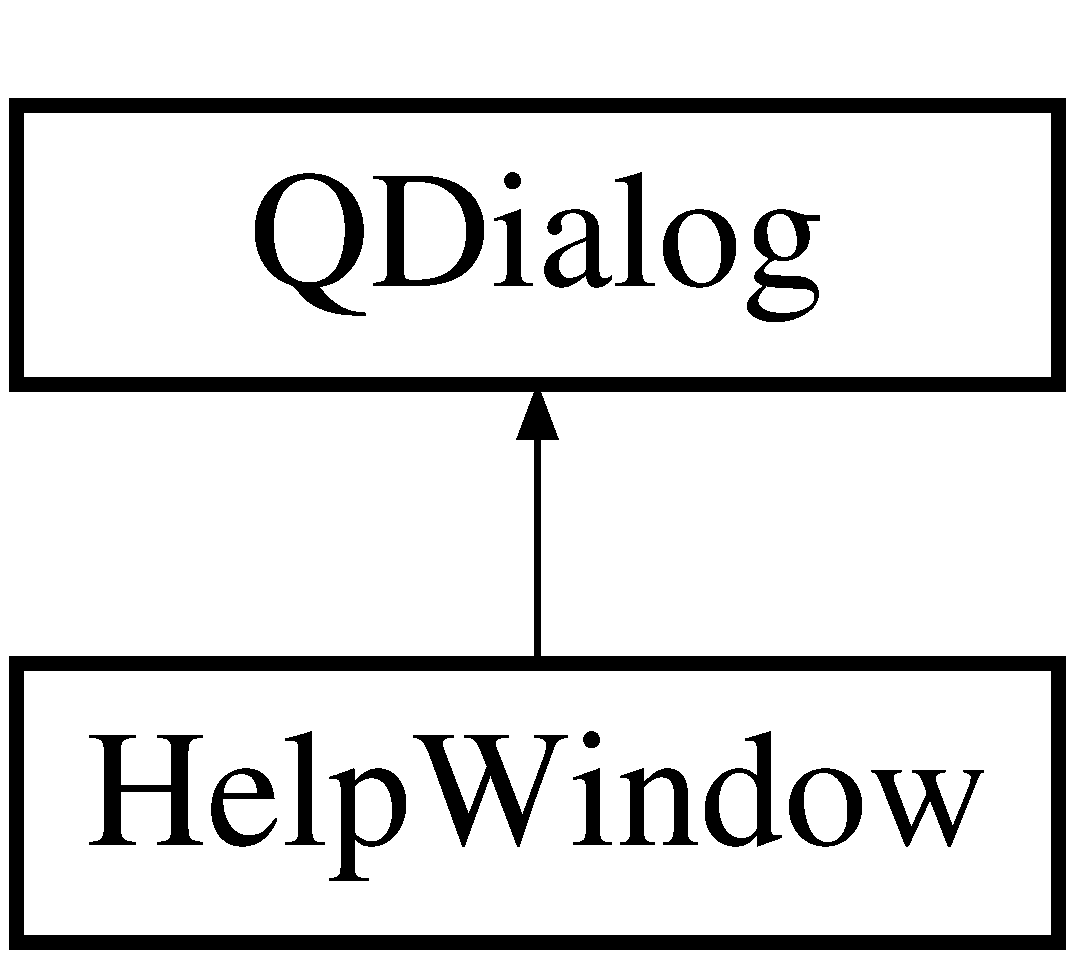
\includegraphics[height=2.000000cm]{class_help_window}
\end{center}
\end{figure}
\subsection*{Public Member Functions}
\begin{DoxyCompactItemize}
\item 
\hypertarget{class_help_window_a9015baabf277f3973dc6028031d57467}{}{\bfseries Help\+Window} (Q\+Widget $\ast$parent=0)\label{class_help_window_a9015baabf277f3973dc6028031d57467}

\end{DoxyCompactItemize}


The documentation for this class was generated from the following files\+:\begin{DoxyCompactItemize}
\item 
helpwindow.\+h\item 
helpwindow.\+cpp\end{DoxyCompactItemize}

\hypertarget{struct_interpreted_data}{}\section{Interpreted\+Data Struct Reference}
\label{struct_interpreted_data}\index{Interpreted\+Data@{Interpreted\+Data}}


The \hyperlink{struct_interpreted_data}{Interpreted\+Data} struct is used to store all interpreted data read from the network.  




{\ttfamily \#include $<$datatypes.\+h$>$}

\subsection*{Public Attributes}
\begin{DoxyCompactItemize}
\item 
\hypertarget{struct_interpreted_data_a575dbb4100a1253cb3e8e2e6a46dd014}{}Q\+Date\+Time {\bfseries timestamp}\label{struct_interpreted_data_a575dbb4100a1253cb3e8e2e6a46dd014}

\item 
\hypertarget{struct_interpreted_data_add4b7dafd9e5bd80ee8600f5cb0c3ed0}{}int {\bfseries Engine\+Switch}\label{struct_interpreted_data_add4b7dafd9e5bd80ee8600f5cb0c3ed0}

\item 
\hypertarget{struct_interpreted_data_afa08eb9585ccf0f7a9424f3dc0d331d7}{}int {\bfseries Master\+Switch}\label{struct_interpreted_data_afa08eb9585ccf0f7a9424f3dc0d331d7}

\item 
\hypertarget{struct_interpreted_data_a0cd97d708630f1fcbd77a3e8a217f3b7}{}int {\bfseries Runlevel\+K60rear}\label{struct_interpreted_data_a0cd97d708630f1fcbd77a3e8a217f3b7}

\item 
\hypertarget{struct_interpreted_data_a2035206f701e9bb511ce4a4b1278d016}{}int {\bfseries Runlevel\+K60front}\label{struct_interpreted_data_a2035206f701e9bb511ce4a4b1278d016}

\item 
\hypertarget{struct_interpreted_data_a6241995c4d6e997a2ef7b9df66f9a23d}{}int {\bfseries rawacceleratorangle}\label{struct_interpreted_data_a6241995c4d6e997a2ef7b9df66f9a23d}

\item 
\hypertarget{struct_interpreted_data_a2efabfd335c25a31d10be9bfab4ad824}{}int {\bfseries rawacceleratorangle\+Gray}\label{struct_interpreted_data_a2efabfd335c25a31d10be9bfab4ad824}

\item 
\hypertarget{struct_interpreted_data_a3f546363132f6eb243f5ee9ccb0e5353}{}int {\bfseries gear}\label{struct_interpreted_data_a3f546363132f6eb243f5ee9ccb0e5353}

\item 
\hypertarget{struct_interpreted_data_a56db6a20c3db45eef4d22a29e8481477}{}int {\bfseries Torque\+Left}\label{struct_interpreted_data_a56db6a20c3db45eef4d22a29e8481477}

\item 
\hypertarget{struct_interpreted_data_a334fb69ebbdb75cfb243a41a86ec6b88}{}int {\bfseries Braking\+Torque\+Left}\label{struct_interpreted_data_a334fb69ebbdb75cfb243a41a86ec6b88}

\item 
\hypertarget{struct_interpreted_data_ad1b890aa1ca72302380a117287bf50dc}{}int {\bfseries Torque\+Right}\label{struct_interpreted_data_ad1b890aa1ca72302380a117287bf50dc}

\item 
\hypertarget{struct_interpreted_data_ae9749fc0e974edd95769ac043ef0bf43}{}int {\bfseries Braking\+Torque\+Right}\label{struct_interpreted_data_ae9749fc0e974edd95769ac043ef0bf43}

\item 
\hypertarget{struct_interpreted_data_a98cca77fe817739c2b3cb2775650c669}{}int {\bfseries errorid\+K60rear}\label{struct_interpreted_data_a98cca77fe817739c2b3cb2775650c669}

\item 
\hypertarget{struct_interpreted_data_a01d435dac22c09f8d9b59bdb7c3cbf9f}{}int {\bfseries errorid\+K60front}\label{struct_interpreted_data_a01d435dac22c09f8d9b59bdb7c3cbf9f}

\item 
\hypertarget{struct_interpreted_data_a3fd4fd5e76f150270d3a9a37ba28d5a4}{}bool {\bfseries Ethernet\+Ok\+Front}\label{struct_interpreted_data_a3fd4fd5e76f150270d3a9a37ba28d5a4}

\item 
\hypertarget{struct_interpreted_data_a83c8124f833f2ae72599d1c078aaceb9}{}bool {\bfseries Ethernet\+Ok\+Rear}\label{struct_interpreted_data_a83c8124f833f2ae72599d1c078aaceb9}

\item 
\hypertarget{struct_interpreted_data_a372456cd1109bc79fb9ee00f8e5d8ed4}{}float {\bfseries Converter\+Left\+Battery\+Current}\label{struct_interpreted_data_a372456cd1109bc79fb9ee00f8e5d8ed4}

\item 
\hypertarget{struct_interpreted_data_a8280d1353b903545477be11cbfd45bf1}{}float {\bfseries Converter\+Left\+Capacitor\+Voltage}\label{struct_interpreted_data_a8280d1353b903545477be11cbfd45bf1}

\item 
\hypertarget{struct_interpreted_data_a4226f87344e8a82bf13a511270467d01}{}float {\bfseries Converter\+Left\+Controller\+Temp}\label{struct_interpreted_data_a4226f87344e8a82bf13a511270467d01}

\item 
\hypertarget{struct_interpreted_data_af4556cf6454e74cf642d299ff7d24a05}{}float {\bfseries Converter\+Left\+Current\+R\+M\+S}\label{struct_interpreted_data_af4556cf6454e74cf642d299ff7d24a05}

\item 
\hypertarget{struct_interpreted_data_a1cb2d6cb24a8cea035549c40af387156}{}float {\bfseries Converter\+Left\+Current\+Request}\label{struct_interpreted_data_a1cb2d6cb24a8cea035549c40af387156}

\item 
\hypertarget{struct_interpreted_data_a94743170c7df0126d98c46452f2b476d}{}int {\bfseries Converter\+Left\+Motor\+R\+P\+M}\label{struct_interpreted_data_a94743170c7df0126d98c46452f2b476d}

\item 
\hypertarget{struct_interpreted_data_acca4e6cf014318fec659b36afc6c3744}{}float {\bfseries Converter\+Left\+Motor\+Temp}\label{struct_interpreted_data_acca4e6cf014318fec659b36afc6c3744}

\item 
\hypertarget{struct_interpreted_data_a9d86736a0a14db7bf93ef0d96631c599}{}float {\bfseries Converter\+Left\+V\+C\+L\+Throttle}\label{struct_interpreted_data_a9d86736a0a14db7bf93ef0d96631c599}

\item 
\hypertarget{struct_interpreted_data_a149bb6f446b5de8e6938ded9ed570066}{}float {\bfseries Converter\+Right\+Battery\+Current}\label{struct_interpreted_data_a149bb6f446b5de8e6938ded9ed570066}

\item 
\hypertarget{struct_interpreted_data_a54586cd17c9630761daa12d6109af5b3}{}float {\bfseries Converter\+Right\+Capacitor\+Voltage}\label{struct_interpreted_data_a54586cd17c9630761daa12d6109af5b3}

\item 
\hypertarget{struct_interpreted_data_ab2223aea7d5fb6a6859e1a0235478ecf}{}float {\bfseries Converter\+Right\+Controller\+Temp}\label{struct_interpreted_data_ab2223aea7d5fb6a6859e1a0235478ecf}

\item 
\hypertarget{struct_interpreted_data_a10619dcab6966a549c369b801008a30a}{}float {\bfseries Converter\+Right\+Current\+R\+M\+S}\label{struct_interpreted_data_a10619dcab6966a549c369b801008a30a}

\item 
\hypertarget{struct_interpreted_data_a201020b272448c8a1876c63b295a8e4a}{}float {\bfseries Converter\+Right\+Current\+Request}\label{struct_interpreted_data_a201020b272448c8a1876c63b295a8e4a}

\item 
\hypertarget{struct_interpreted_data_a9e2cc54e88300b45644d1176f14ab4be}{}int {\bfseries Converter\+Right\+Motor\+R\+P\+M}\label{struct_interpreted_data_a9e2cc54e88300b45644d1176f14ab4be}

\item 
\hypertarget{struct_interpreted_data_adf18cb1cf5770fd5dcf6fe01bf316c68}{}float {\bfseries Converter\+Right\+Motor\+Temp}\label{struct_interpreted_data_adf18cb1cf5770fd5dcf6fe01bf316c68}

\item 
\hypertarget{struct_interpreted_data_a4a29afcd76161d20fc510d8d8e590fe1}{}float {\bfseries Converter\+Right\+V\+C\+L\+Throttle}\label{struct_interpreted_data_a4a29afcd76161d20fc510d8d8e590fe1}

\item 
\hypertarget{struct_interpreted_data_af7fc398919d3d581e326dfbae0286000}{}float {\bfseries D\+C\+D\+Ccurrent}\label{struct_interpreted_data_af7fc398919d3d581e326dfbae0286000}

\item 
\hypertarget{struct_interpreted_data_abfeead79d90093250bea7f8b56d7ed01}{}float {\bfseries H\+V\+V}\label{struct_interpreted_data_abfeead79d90093250bea7f8b56d7ed01}

\item 
\hypertarget{struct_interpreted_data_a97d01dc42903c5fc12de9017b712f9fd}{}bool {\bfseries Direction\+Left}\label{struct_interpreted_data_a97d01dc42903c5fc12de9017b712f9fd}

\item 
\hypertarget{struct_interpreted_data_a99365f8d6fcc330b29ed9a0f9b32c15e}{}bool {\bfseries Direction\+Right}\label{struct_interpreted_data_a99365f8d6fcc330b29ed9a0f9b32c15e}

\item 
\hypertarget{struct_interpreted_data_a6934078968c49dc5cb9401f7d0fe4a92}{}bool {\bfseries Horn}\label{struct_interpreted_data_a6934078968c49dc5cb9401f7d0fe4a92}

\item 
\hypertarget{struct_interpreted_data_a48b571c876225661e166a68b6d1d586f}{}bool {\bfseries Backward\+Light}\label{struct_interpreted_data_a48b571c876225661e166a68b6d1d586f}

\item 
\hypertarget{struct_interpreted_data_a64271b71324461681cdf1bb1b796314d}{}bool {\bfseries Brake\+Light}\label{struct_interpreted_data_a64271b71324461681cdf1bb1b796314d}

\item 
\hypertarget{struct_interpreted_data_ad3c1b3fd572270f350ea6bd6abe3f11e}{}bool {\bfseries Forward\+Light}\label{struct_interpreted_data_ad3c1b3fd572270f350ea6bd6abe3f11e}

\item 
\hypertarget{struct_interpreted_data_ad24aa791e12fdf619e996051d3f20dd0}{}bool {\bfseries Warning\+Light}\label{struct_interpreted_data_ad24aa791e12fdf619e996051d3f20dd0}

\item 
\hypertarget{struct_interpreted_data_aa909db8cbc53d9b334e89da2a0969fb6}{}bool {\bfseries Full\+Beam\+Light}\label{struct_interpreted_data_aa909db8cbc53d9b334e89da2a0969fb6}

\item 
\hypertarget{struct_interpreted_data_a81b2e046f7ab276255a5adc3ce0bb1f5}{}double {\bfseries speed}\label{struct_interpreted_data_a81b2e046f7ab276255a5adc3ce0bb1f5}

\item 
\hypertarget{struct_interpreted_data_ae45fa4c958b9bc9620597ff99bb855ad}{}double {\bfseries acceleratorpercentage}\label{struct_interpreted_data_ae45fa4c958b9bc9620597ff99bb855ad}

\item 
\hypertarget{struct_interpreted_data_a9813c78f37454855119b91563103cda2}{}double {\bfseries brakepercentage}\label{struct_interpreted_data_a9813c78f37454855119b91563103cda2}

\item 
\hypertarget{struct_interpreted_data_a8026995a500f48ec2745d46b89245f64}{}int {\bfseries S\+O\+C}\label{struct_interpreted_data_a8026995a500f48ec2745d46b89245f64}

\item 
\hypertarget{struct_interpreted_data_af4b484f8a7928d1bd77a953c6cf3db2a}{}int {\bfseries range\+\_\+for\+\_\+\+C\+A\+N}\label{struct_interpreted_data_af4b484f8a7928d1bd77a953c6cf3db2a}

\item 
\hypertarget{struct_interpreted_data_a1752daef53297e84379b2726186b6f5e}{}int {\bfseries S\+P\+I\+\_\+error}\label{struct_interpreted_data_a1752daef53297e84379b2726186b6f5e}

\item 
\hypertarget{struct_interpreted_data_a9542ad91bfcea58a33274e03e90c5c24}{}int {\bfseries S\+P\+I\+\_\+log}\label{struct_interpreted_data_a9542ad91bfcea58a33274e03e90c5c24}

\item 
\hypertarget{struct_interpreted_data_aa1eb54a744b54e049177115754c403b2}{}int {\bfseries B\+M\+S\+\_\+\+Errors}\label{struct_interpreted_data_aa1eb54a744b54e049177115754c403b2}

\item 
\hypertarget{struct_interpreted_data_a1556b57ee2fc637cb7bfbed08e487160}{}int {\bfseries S\+H\+U\+N\+T\+\_\+error}\label{struct_interpreted_data_a1556b57ee2fc637cb7bfbed08e487160}

\item 
\hypertarget{struct_interpreted_data_af99ef02156b7f3d9283396375be05329}{}int {\bfseries R\+E\+L\+A\+Y\+\_\+enable}\label{struct_interpreted_data_af99ef02156b7f3d9283396375be05329}

\item 
\hypertarget{struct_interpreted_data_a1276de85e0d0a059af02cdccbf7e6511}{}int {\bfseries current\+\_\+for\+\_\+\+C\+A\+N}\label{struct_interpreted_data_a1276de85e0d0a059af02cdccbf7e6511}

\item 
\hypertarget{struct_interpreted_data_af76daadb1de6429ee9eddeb56189397a}{}int {\bfseries voltage\+\_\+\+Stack\+\_\+for\+\_\+\+C\+A\+N}\label{struct_interpreted_data_af76daadb1de6429ee9eddeb56189397a}

\item 
\hypertarget{struct_interpreted_data_a383ac191f4a1e3f2456b06ce7d0c4577}{}int {\bfseries voltage\+\_\+cell\+\_\+highest\+\_\+for\+\_\+\+C\+A\+N}\label{struct_interpreted_data_a383ac191f4a1e3f2456b06ce7d0c4577}

\item 
\hypertarget{struct_interpreted_data_adcfde647393b5e1f1ffec5326cd8f89a}{}int {\bfseries voltage\+\_\+cell\+\_\+lowest\+\_\+for\+\_\+\+C\+A\+N}\label{struct_interpreted_data_adcfde647393b5e1f1ffec5326cd8f89a}

\item 
\hypertarget{struct_interpreted_data_a67175722e02b00f8f3b2c8b25eaf2e67}{}int {\bfseries max\+\_\+\+Temp}\label{struct_interpreted_data_a67175722e02b00f8f3b2c8b25eaf2e67}

\item 
\hypertarget{struct_interpreted_data_ab85950943a2912a8f879b99342505365}{}int {\bfseries battery\+\_\+cell} \mbox{[}16\mbox{]}\label{struct_interpreted_data_ab85950943a2912a8f879b99342505365}

\end{DoxyCompactItemize}


\subsection{Detailed Description}
The \hyperlink{struct_interpreted_data}{Interpreted\+Data} struct is used to store all interpreted data read from the network. 

The documentation for this struct was generated from the following file\+:\begin{DoxyCompactItemize}
\item 
datatypes.\+h\end{DoxyCompactItemize}

\hypertarget{class_interprete_thread}{}\section{Interprete\+Thread Class Reference}
\label{class_interprete_thread}\index{Interprete\+Thread@{Interprete\+Thread}}


The \hyperlink{class_interprete_thread}{Interprete\+Thread} class interpretes the incoming U\+D\+P messages. Messages with known I\+D\textquotesingle{}s are saved to Latest\+Data\+Interpreted. Each message will be saved to the vector Latest\+Raw\+Data and the data log will be saved in Interpreted\+History and Raw\+History.  




{\ttfamily \#include $<$interpretethread.\+h$>$}

Inheritance diagram for Interprete\+Thread\+:\begin{figure}[H]
\begin{center}
\leavevmode
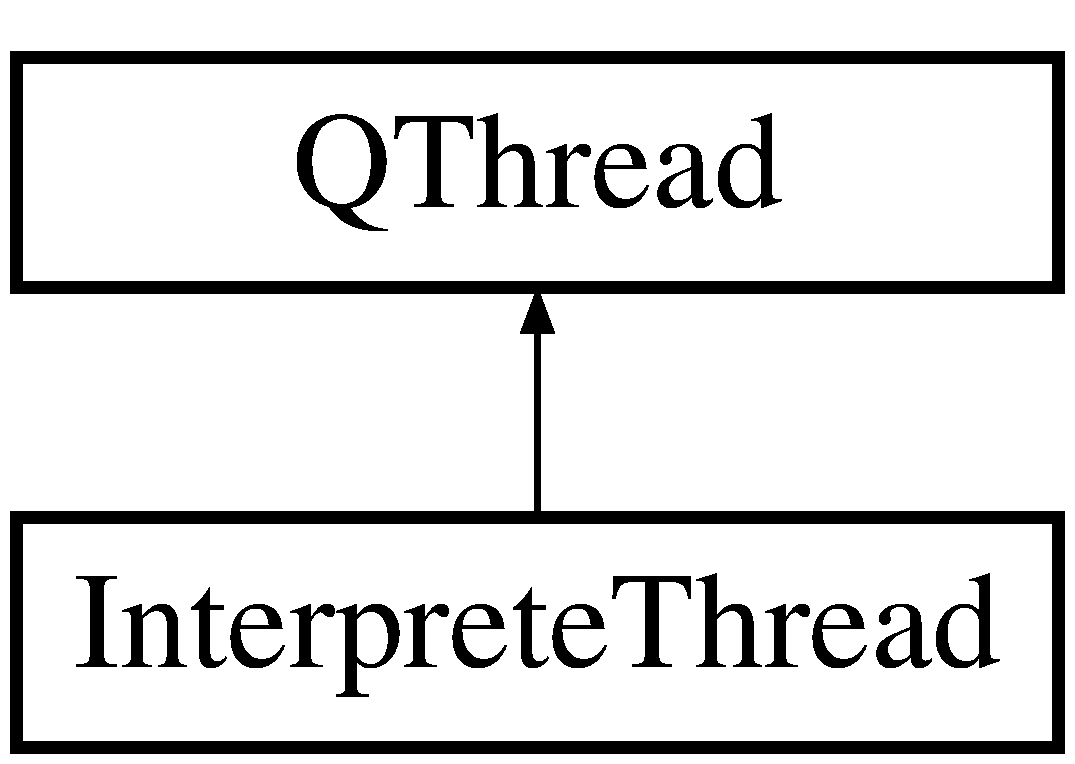
\includegraphics[height=2.000000cm]{class_interprete_thread}
\end{center}
\end{figure}
\subsection*{Public Member Functions}
\begin{DoxyCompactItemize}
\item 
\hypertarget{class_interprete_thread_ab0a4b3eed2973554a85ae62069da0830}{}{\bfseries Interprete\+Thread} (Q\+Object $\ast$parent=0)\label{class_interprete_thread_ab0a4b3eed2973554a85ae62069da0830}

\item 
void \hyperlink{class_interprete_thread_a9e2e7ed3a9608daa29393850ce380ffc}{Daten\+\_\+konvertieren} (\hyperlink{struct_ethernet___msg}{Ethernet\+\_\+\+Msg} Msg)
\begin{DoxyCompactList}\small\item\em Daten\+\_\+konvertieren. \end{DoxyCompactList}\item 
\hypertarget{class_interprete_thread_ad5a48ad3b85aefb7bff76414589fa5a5}{}void {\bfseries Interprete\+From\+Json} (\hyperlink{struct_ethernet___msg}{Ethernet\+\_\+\+Msg} Msg)\label{class_interprete_thread_ad5a48ad3b85aefb7bff76414589fa5a5}

\item 
\hypertarget{class_interprete_thread_aeaac0ccd7cc19a774c328ecef95c7e76}{}void {\bfseries init\+\_\+\+Latest\+Data\+Interpreted} (struct \hyperlink{struct_interpreted_data}{Interpreted\+Data} $\ast$)\label{class_interprete_thread_aeaac0ccd7cc19a774c328ecef95c7e76}

\item 
\hypertarget{class_interprete_thread_a9106a12f445bf84eccf5c5dd3aabacb0}{}void {\bfseries init\+\_\+received\+Msg\+Vector} (std\+::vector$<$ \hyperlink{struct_ethernet___msg}{Ethernet\+\_\+\+Msg} $>$ $\ast$)\label{class_interprete_thread_a9106a12f445bf84eccf5c5dd3aabacb0}

\item 
\hypertarget{class_interprete_thread_a0b7d95389d386788d95764e244c87deb}{}void {\bfseries init\+\_\+\+Latest\+Raw\+Data} (struct \hyperlink{struct_raw_data}{Raw\+Data} $\ast$)\label{class_interprete_thread_a0b7d95389d386788d95764e244c87deb}

\item 
\hypertarget{class_interprete_thread_ada92262f4fe1ec478be5b023693e4e65}{}void {\bfseries init\+\_\+\+Available\+Data} (int $\ast$)\label{class_interprete_thread_ada92262f4fe1ec478be5b023693e4e65}

\end{DoxyCompactItemize}
\subsection*{Public Attributes}
\begin{DoxyCompactItemize}
\item 
\hypertarget{class_interprete_thread_ac7fbde461d6471d864605143cd77b27d}{}bool {\bfseries rearok}\label{class_interprete_thread_ac7fbde461d6471d864605143cd77b27d}

\item 
\hypertarget{class_interprete_thread_aaf773375f45a30ea052af1a05a31b9df}{}bool {\bfseries frontok}\label{class_interprete_thread_aaf773375f45a30ea052af1a05a31b9df}

\end{DoxyCompactItemize}
\subsection*{Protected Member Functions}
\begin{DoxyCompactItemize}
\item 
\hypertarget{class_interprete_thread_aa24b72df0d69cf668ae26919a6cafc58}{}void \hyperlink{class_interprete_thread_aa24b72df0d69cf668ae26919a6cafc58}{run} ()\label{class_interprete_thread_aa24b72df0d69cf668ae26919a6cafc58}

\begin{DoxyCompactList}\small\item\em \hyperlink{class_interprete_thread_aa24b72df0d69cf668ae26919a6cafc58}{run()} -\/\+Main function. will loop as long as the thread is not terminated. -\/\+It dequeues the messages from the Queue Rec\+Queue and convertes them\+: \hyperlink{struct_recv_buf}{Recv\+Buf} to \hyperlink{struct_ethernet___msg}{Ethernet\+\_\+\+Msg} -\/\+Does the interpretation and displaying by calling the needed functions. -\/\+Data will be saved in the Latest\+Raw\+Data vector -\/\+The interpretation is the task of \hyperlink{class_interprete_thread_a9e2e7ed3a9608daa29393850ce380ffc}{Daten\+\_\+konvertieren(\+Ethernet\+\_\+\+Msg msg)} -\/\+The data log will be saved in Interpreted\+History and Raw\+History \end{DoxyCompactList}\end{DoxyCompactItemize}


\subsection{Detailed Description}
The \hyperlink{class_interprete_thread}{Interprete\+Thread} class interpretes the incoming U\+D\+P messages. Messages with known I\+D\textquotesingle{}s are saved to Latest\+Data\+Interpreted. Each message will be saved to the vector Latest\+Raw\+Data and the data log will be saved in Interpreted\+History and Raw\+History. 

\subsection{Member Function Documentation}
\hypertarget{class_interprete_thread_a9e2e7ed3a9608daa29393850ce380ffc}{}\index{Interprete\+Thread@{Interprete\+Thread}!Daten\+\_\+konvertieren@{Daten\+\_\+konvertieren}}
\index{Daten\+\_\+konvertieren@{Daten\+\_\+konvertieren}!Interprete\+Thread@{Interprete\+Thread}}
\subsubsection[{Daten\+\_\+konvertieren(\+Ethernet\+\_\+\+Msg Msg)}]{\setlength{\rightskip}{0pt plus 5cm}void Interprete\+Thread\+::\+Daten\+\_\+konvertieren (
\begin{DoxyParamCaption}
\item[{{\bf Ethernet\+\_\+\+Msg}}]{Msg}
\end{DoxyParamCaption}
)}\label{class_interprete_thread_a9e2e7ed3a9608daa29393850ce380ffc}


Daten\+\_\+konvertieren. 


\begin{DoxyParams}{Parameters}
{\em } & \\
\hline
\end{DoxyParams}


The documentation for this class was generated from the following files\+:\begin{DoxyCompactItemize}
\item 
interpretethread.\+h\item 
interpretethread.\+cpp\end{DoxyCompactItemize}

\hypertarget{struct_log_command}{}\section{Log\+Command Struct Reference}
\label{struct_log_command}\index{Log\+Command@{Log\+Command}}


The documentation for this struct was generated from the following file\+:\begin{DoxyCompactItemize}
\item 
datatypes.\+h\end{DoxyCompactItemize}

\hypertarget{class_main_window}{}\section{Main\+Window Class Reference}
\label{class_main_window}\index{Main\+Window@{Main\+Window}}
Inheritance diagram for Main\+Window\+:\begin{figure}[H]
\begin{center}
\leavevmode
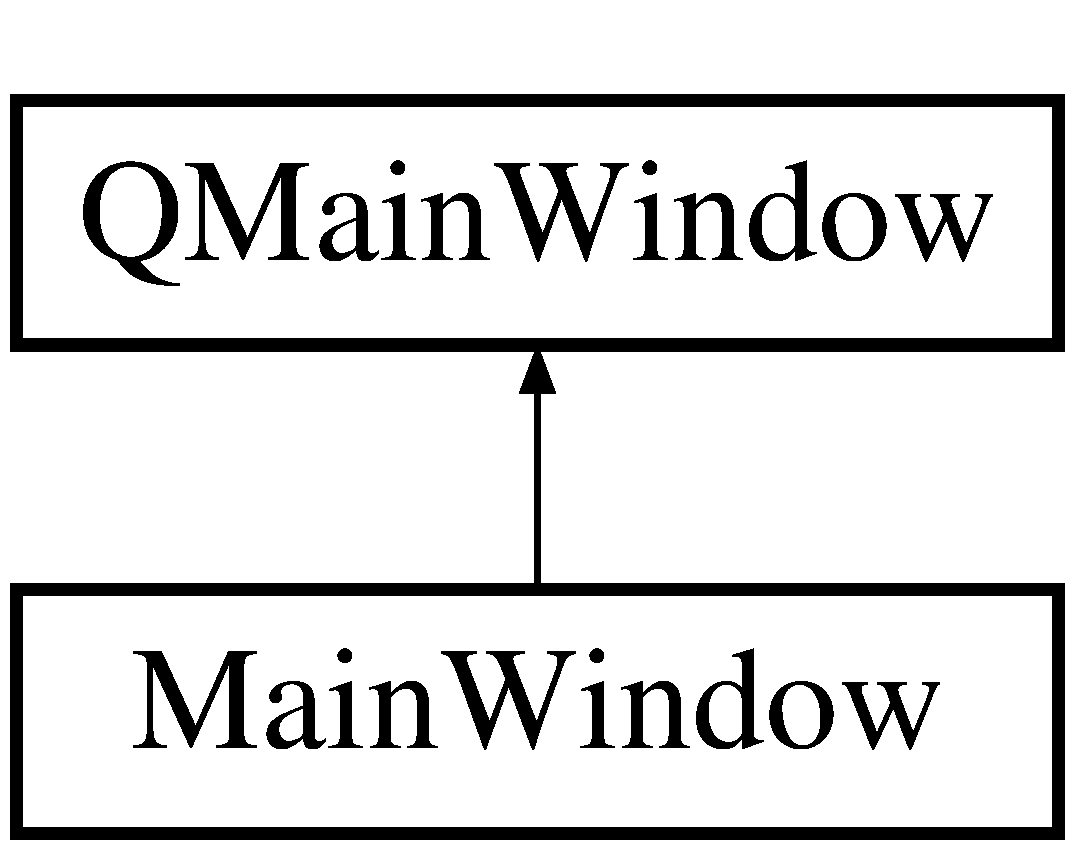
\includegraphics[height=2.000000cm]{class_main_window}
\end{center}
\end{figure}
\subsection*{Public Slots}
\begin{DoxyCompactItemize}
\item 
void \hyperlink{class_main_window_a042e863e901d40459d15a354ee4f9283}{Update\+Gui} ()
\begin{DoxyCompactList}\small\item\em Update\+Gui updates elements of the G\+U\+I every 100ms. \end{DoxyCompactList}\item 
\hypertarget{class_main_window_a3a9f39d07cb3fe42a152c05757c1da5a}{}void {\bfseries Change\+Gear\+List} (int)\label{class_main_window_a3a9f39d07cb3fe42a152c05757c1da5a}

\item 
\hypertarget{class_main_window_acd5aa2271fa4b95c8e315ea08e1ded23}{}void {\bfseries Change\+Gear\+List\+\_\+\+Released} (int)\label{class_main_window_acd5aa2271fa4b95c8e315ea08e1ded23}

\item 
\hypertarget{class_main_window_a5d07507433b877fab2041feb43a118aa}{}void {\bfseries on\+\_\+\+Connect\+\_\+\+Button\+\_\+clicked} (void)\label{class_main_window_a5d07507433b877fab2041feb43a118aa}

\item 
\hypertarget{class_main_window_a60ca4a58bd344915de9e4f3c4e56c15c}{}void \hyperlink{class_main_window_a60ca4a58bd344915de9e4f3c4e56c15c}{on\+\_\+start\+Remote\+Button\+\_\+clicked} (void)\label{class_main_window_a60ca4a58bd344915de9e4f3c4e56c15c}

\begin{DoxyCompactList}\small\item\em activates the remote control and setups connections to the remote thread \end{DoxyCompactList}\item 
\hypertarget{class_main_window_a7769c1b0723c2827f6cbcbc571c1d6d7}{}void {\bfseries on\+\_\+stop\+Remote\+Button\+\_\+clicked} (void)\label{class_main_window_a7769c1b0723c2827f6cbcbc571c1d6d7}

\item 
\hypertarget{class_main_window_adefd278b8a51511b1b7739f1fba58182}{}void {\bfseries on\+\_\+warning\+Button\+\_\+clicked} (void)\label{class_main_window_adefd278b8a51511b1b7739f1fba58182}

\item 
\hypertarget{class_main_window_aaba0478e64701fa9b96670c89f294e44}{}void {\bfseries on\+\_\+warning\+Button\+\_\+\+Released} (void)\label{class_main_window_aaba0478e64701fa9b96670c89f294e44}

\item 
\hypertarget{class_main_window_a700c75646dc095274f6243a3839103b0}{}void {\bfseries on\+\_\+indicator\+Right\+Button\+\_\+clicked} (void)\label{class_main_window_a700c75646dc095274f6243a3839103b0}

\item 
\hypertarget{class_main_window_a16b416264054c670d9d99a71557d6170}{}void {\bfseries on\+\_\+indicator\+Right\+Button\+\_\+\+Released} (void)\label{class_main_window_a16b416264054c670d9d99a71557d6170}

\item 
\hypertarget{class_main_window_ace1c4f24a9c967088bf0bdbe2e8c0016}{}void {\bfseries on\+\_\+indicator\+Left\+Button\+\_\+clicked} (void)\label{class_main_window_ace1c4f24a9c967088bf0bdbe2e8c0016}

\item 
\hypertarget{class_main_window_ac5b52146cdc9b0f800e297e6878e5b64}{}void {\bfseries on\+\_\+indicator\+Left\+Button\+\_\+\+Released} (void)\label{class_main_window_ac5b52146cdc9b0f800e297e6878e5b64}

\item 
\hypertarget{class_main_window_a83da26aea6092b16af47b168934d0b53}{}void {\bfseries on\+\_\+full\+Beam\+Button\+\_\+clicked} (void)\label{class_main_window_a83da26aea6092b16af47b168934d0b53}

\item 
\hypertarget{class_main_window_a6b9b4805bed75625acf7173ca1aa2b51}{}void {\bfseries on\+\_\+full\+Beam\+Button\+\_\+\+Released} (void)\label{class_main_window_a6b9b4805bed75625acf7173ca1aa2b51}

\item 
\hypertarget{class_main_window_ac42ccb3fdc4d023d24a96f6ef2b8a276}{}void {\bfseries on\+\_\+head\+Light\+Button\+\_\+clicked} (void)\label{class_main_window_ac42ccb3fdc4d023d24a96f6ef2b8a276}

\item 
\hypertarget{class_main_window_a85a881ef94e347bdd8272880ad62d625}{}void {\bfseries on\+\_\+head\+Light\+Button\+\_\+\+Released} (void)\label{class_main_window_a85a881ef94e347bdd8272880ad62d625}

\item 
\hypertarget{class_main_window_a9bd9f4929af22bf0b859941e8ed2138f}{}void {\bfseries on\+\_\+brake\+Button\+\_\+clicked} (int)\label{class_main_window_a9bd9f4929af22bf0b859941e8ed2138f}

\item 
\hypertarget{class_main_window_a0c692b460f19ba18bc73995e963cd153}{}void {\bfseries on\+\_\+accelerate\+Button\+\_\+clicked} (int)\label{class_main_window_a0c692b460f19ba18bc73995e963cd153}

\item 
\hypertarget{class_main_window_abe4b8da14328af4d591d714685f19164}{}void {\bfseries on\+\_\+horn\+Button\+\_\+clicked} (void)\label{class_main_window_abe4b8da14328af4d591d714685f19164}

\item 
\hypertarget{class_main_window_aa42039e574e036e640ab9e20ab08e7a2}{}void {\bfseries on\+\_\+horn\+Button\+\_\+\+Released} (void)\label{class_main_window_aa42039e574e036e640ab9e20ab08e7a2}

\item 
\hypertarget{class_main_window_a0a589c017e8858f2856ecf198f2762e1}{}void {\bfseries on\+\_\+steering} (int)\label{class_main_window_a0a589c017e8858f2856ecf198f2762e1}

\item 
\hypertarget{class_main_window_a693c95d5a5393f1d49497e82502c4ead}{}void {\bfseries arrive\+\_\+\+Animation\+\_\+finished} ()\label{class_main_window_a693c95d5a5393f1d49497e82502c4ead}

\item 
\hypertarget{class_main_window_aa17d087c9affe02c39bd9b71f1bddf0e}{}void {\bfseries depart\+\_\+\+Animation\+\_\+finished} ()\label{class_main_window_aa17d087c9affe02c39bd9b71f1bddf0e}

\item 
\hypertarget{class_main_window_af17fda29d8ac7e4afe9b311b716e12ce}{}void {\bfseries on\+\_\+help\+Window\+Mouse\+Entered} ()\label{class_main_window_af17fda29d8ac7e4afe9b311b716e12ce}

\item 
\hypertarget{class_main_window_a3157573a5834a4e1bd4ab73f9a1376b7}{}void {\bfseries on\+\_\+help\+Window\+Mouse\+Leaved} ()\label{class_main_window_a3157573a5834a4e1bd4ab73f9a1376b7}

\item 
\hypertarget{class_main_window_ae009b2d1ec85c5f757b179ae6ee2e0cb}{}void {\bfseries on\+\_\+help\+Window\+Mouse\+Clicked} ()\label{class_main_window_ae009b2d1ec85c5f757b179ae6ee2e0cb}

\item 
\hypertarget{class_main_window_a108aeb29eb7f25a6e578428f39fc2d9b}{}void {\bfseries on\+\_\+ethernet\+A\+A\+Radio\+Button\+\_\+clicked} ()\label{class_main_window_a108aeb29eb7f25a6e578428f39fc2d9b}

\item 
\hypertarget{class_main_window_ab05ccc37a4f37cb0078ae583055006b2}{}void {\bfseries on\+\_\+ethernet\+Custom\+Radio\+Button\+\_\+clicked} ()\label{class_main_window_ab05ccc37a4f37cb0078ae583055006b2}

\item 
\hypertarget{class_main_window_ab61a70cb62b2bc922ac479f23a88e50d}{}void {\bfseries on\+\_\+checksum\+Compute\+Radio\+Button\+\_\+clicked} ()\label{class_main_window_ab61a70cb62b2bc922ac479f23a88e50d}

\item 
\hypertarget{class_main_window_a62373ed1ad6a163e38690852a27a4851}{}void {\bfseries on\+\_\+checksum\+Custom\+Radio\+Button\+\_\+clicked} ()\label{class_main_window_a62373ed1ad6a163e38690852a27a4851}

\item 
\hypertarget{class_main_window_a93b971f29c7a801b978860c72621c75f}{}void \hyperlink{class_main_window_a93b971f29c7a801b978860c72621c75f}{on\+\_\+\+Debug\+Send\+Now\+Button\+\_\+clicked} ()\label{class_main_window_a93b971f29c7a801b978860c72621c75f}

\begin{DoxyCompactList}\small\item\em on\+\_\+\+Debug\+Send\+Now\+Button\+\_\+clicked This function allows the user to either enter a ethernet message that will be sent or to enter a can message and set all settings to automaticaly generate a ethernet message that will be sent. \end{DoxyCompactList}\item 
\hypertarget{class_main_window_aa23d984401f68b77a3ad4f86c066772d}{}void {\bfseries on\+\_\+\+Debug\+Add\+Button\+\_\+clicked} ()\label{class_main_window_aa23d984401f68b77a3ad4f86c066772d}

\item 
\hypertarget{class_main_window_aeb03be7f76187eb6cf15b0040aee2d29}{}void {\bfseries on\+\_\+\+Debug\+Toggle\+Active\+Button\+\_\+clicked} ()\label{class_main_window_aeb03be7f76187eb6cf15b0040aee2d29}

\item 
\hypertarget{class_main_window_affaa67dd793fb6c2f891d026655b70cc}{}void {\bfseries on\+\_\+\+Debug\+Remove\+Button\+\_\+clicked} ()\label{class_main_window_affaa67dd793fb6c2f891d026655b70cc}

\item 
\hypertarget{class_main_window_acc524496197c940e49d6ff80a134bd29}{}void {\bfseries on\+\_\+\+Debug\+Enable\+Check\+Box\+\_\+clicked} ()\label{class_main_window_acc524496197c940e49d6ff80a134bd29}

\item 
\hypertarget{class_main_window_a472c3d7b7542bcf87d59f1953b27283b}{}void {\bfseries on\+\_\+\+Debug\+Manual\+Radio\+Button\+\_\+clicked} ()\label{class_main_window_a472c3d7b7542bcf87d59f1953b27283b}

\item 
\hypertarget{class_main_window_ad7d84560f6cf5ab723151ba7b239f237}{}void {\bfseries on\+\_\+\+Debug\+Guided\+Radio\+Button\+\_\+clicked} ()\label{class_main_window_ad7d84560f6cf5ab723151ba7b239f237}

\item 
\hypertarget{class_main_window_a7bf06b12acdc55f1a3077e075ddc1368}{}void {\bfseries on\+\_\+\+Debug\+None\+Radio\+Button\+\_\+clicked} ()\label{class_main_window_a7bf06b12acdc55f1a3077e075ddc1368}

\item 
\hypertarget{class_main_window_a2fd364f1604f4a82b6d184e2cfee0546}{}void {\bfseries on\+\_\+mode\+Combo\+Box\+\_\+current\+Index\+Changed} (int index)\label{class_main_window_a2fd364f1604f4a82b6d184e2cfee0546}

\item 
\hypertarget{class_main_window_aea9eea589a148ada379206476661b925}{}void {\bfseries on\+\_\+recup\+Combo\+Box\+\_\+current\+Index\+Changed} (int index)\label{class_main_window_aea9eea589a148ada379206476661b925}

\item 
\hypertarget{class_main_window_adc3aedfd4752bea231cfe467eb3543ff}{}void {\bfseries on\+\_\+boost\+Combo\+Box\+\_\+current\+Index\+Changed} (int index)\label{class_main_window_adc3aedfd4752bea231cfe467eb3543ff}

\item 
\hypertarget{class_main_window_a42075b4c9053cc3143e0bcafc1fea0ff}{}void {\bfseries on\+\_\+\+C\+A\+L\+\_\+\+Start\+Button\+\_\+clicked} ()\label{class_main_window_a42075b4c9053cc3143e0bcafc1fea0ff}

\item 
\hypertarget{class_main_window_ae5a5d073e5ef686fe22c50c49752da96}{}void {\bfseries on\+\_\+\+C\+A\+L\+\_\+\+Continue\+Button\+\_\+clicked} ()\label{class_main_window_ae5a5d073e5ef686fe22c50c49752da96}

\item 
\hypertarget{class_main_window_a251135c1f48fa30ac11aa85a039a7b0d}{}void {\bfseries on\+\_\+\+Create\+Log\+Button\+\_\+clicked} ()\label{class_main_window_a251135c1f48fa30ac11aa85a039a7b0d}

\item 
\hypertarget{class_main_window_ab2383fd202337a140d03dea789351376}{}void {\bfseries on\+\_\+max\+Speed\+Slider\+\_\+action\+Triggered} (int action)\label{class_main_window_ab2383fd202337a140d03dea789351376}

\item 
\hypertarget{class_main_window_a767ec2866317dfbdcc48dafa1864af4d}{}void {\bfseries on\+\_\+max\+Speed\+Slider\+\_\+slider\+Moved} (int position)\label{class_main_window_a767ec2866317dfbdcc48dafa1864af4d}

\item 
void \hyperlink{class_main_window_abf516f6eaf5bff5bbd76449f5c0d63ef}{on\+\_\+max\+Speed\+Slider\+\_\+value\+Changed} (int value)
\begin{DoxyCompactList}\small\item\em called when the value of the slider changes \end{DoxyCompactList}\item 
\hypertarget{class_main_window_aa68eba140c2cf5c1cd2b4bd81337fa83}{}void {\bfseries on\+\_\+action\+Quit\+\_\+triggered} ()\label{class_main_window_aa68eba140c2cf5c1cd2b4bd81337fa83}

\item 
\hypertarget{class_main_window_aad8b3565829ef596ac57aa46253b306b}{}void \hyperlink{class_main_window_aad8b3565829ef596ac57aa46253b306b}{on\+\_\+action\+Get\+\_\+\+Help\+\_\+triggered} ()\label{class_main_window_aad8b3565829ef596ac57aa46253b306b}

\begin{DoxyCompactList}\small\item\em \hyperlink{class_main_window_aad8b3565829ef596ac57aa46253b306b}{Main\+Window\+::on\+\_\+action\+Get\+\_\+\+Help\+\_\+triggered} ( it opens a H\+T\+M\+L page ( Help Window) ) \end{DoxyCompactList}\item 
\hypertarget{class_main_window_a4f3ebda1ba39e0ef4d678b44893c9c7f}{}void {\bfseries on\+\_\+action\+About\+\_\+triggered} ()\label{class_main_window_a4f3ebda1ba39e0ef4d678b44893c9c7f}

\item 
\hypertarget{class_main_window_a4bb83ab10a82172751db9f859a605016}{}void \hyperlink{class_main_window_a4bb83ab10a82172751db9f859a605016}{on\+\_\+action\+Connect\+\_\+\+Disconnect\+\_\+triggered} ()\label{class_main_window_a4bb83ab10a82172751db9f859a605016}

\begin{DoxyCompactList}\small\item\em \hyperlink{class_main_window_a4bb83ab10a82172751db9f859a605016}{Main\+Window\+::on\+\_\+action\+Connect\+\_\+\+Disconnect\+\_\+triggered} \+: called to verify if there is connection with the car or not. \end{DoxyCompactList}\item 
\hypertarget{class_main_window_a1c2ee7f6950fb7b597549563d002111e}{}void {\bfseries on\+\_\+\+Development\+\_\+\+Button\+\_\+clicked} ()\label{class_main_window_a1c2ee7f6950fb7b597549563d002111e}

\item 
\hypertarget{class_main_window_a4de79c63c7fa0b8d7c468ac71f20be81}{}void {\bfseries on\+\_\+push\+Button\+\_\+clicked} ()\label{class_main_window_a4de79c63c7fa0b8d7c468ac71f20be81}

\item 
\hypertarget{class_main_window_afbcef9f3e5a68f8709c86299b0f5d6a9}{}void {\bfseries on\+\_\+horizontal\+Slider\+\_\+value\+Changed} (int value)\label{class_main_window_afbcef9f3e5a68f8709c86299b0f5d6a9}

\item 
\hypertarget{class_main_window_a3f9d31ee127119a82b48c230d38f3c5f}{}void {\bfseries on\+\_\+key\+Assignment\+\_\+\+Button\+\_\+clicked} ()\label{class_main_window_a3f9d31ee127119a82b48c230d38f3c5f}

\end{DoxyCompactItemize}
\subsection*{Public Member Functions}
\begin{DoxyCompactItemize}
\item 
\hypertarget{class_main_window_a8b244be8b7b7db1b08de2a2acb9409db}{}{\bfseries Main\+Window} (Q\+Widget $\ast$parent=0)\label{class_main_window_a8b244be8b7b7db1b08de2a2acb9409db}

\item 
\hypertarget{class_main_window_a4e90dae9d28e99e1a2a708eaf881c485}{}int {\bfseries D\+M\+X\+\_\+\+Send} (int Kanal, unsigned char Wert)\label{class_main_window_a4e90dae9d28e99e1a2a708eaf881c485}

\item 
\hypertarget{class_main_window_a38edb88d43e844aca9d2e762c8706565}{}void {\bfseries close\+Event} (Q\+Close\+Event $\ast$)\label{class_main_window_a38edb88d43e844aca9d2e762c8706565}

\item 
\hypertarget{class_main_window_ac3b886aa8279a5f084d3568b35bdbeb2}{}void \hyperlink{class_main_window_ac3b886aa8279a5f084d3568b35bdbeb2}{needle\+Rotate} (int)\label{class_main_window_ac3b886aa8279a5f084d3568b35bdbeb2}

\begin{DoxyCompactList}\small\item\em rotates the speedometer\textquotesingle{}s needle depending on the passed speed paramater \end{DoxyCompactList}\item 
\hypertarget{class_main_window_a23b80f82a61cc0a1e3e2721891c782b8}{}void \hyperlink{class_main_window_a23b80f82a61cc0a1e3e2721891c782b8}{tires\+Rotate} (int)\label{class_main_window_a23b80f82a61cc0a1e3e2721891c782b8}

\begin{DoxyCompactList}\small\item\em rotates e\+C\+A\+Rus\textquotesingle{} tires depending on the passed steering value \end{DoxyCompactList}\item 
\hypertarget{class_main_window_a0e5b89d0f15feab33a7c1fb56b398297}{}void {\bfseries arrive\+\_\+\+Animation} ()\label{class_main_window_a0e5b89d0f15feab33a7c1fb56b398297}

\item 
\hypertarget{class_main_window_a0045f76b77a2fda750ce2bd30f8a0a59}{}void {\bfseries depart\+\_\+\+Animation} ()\label{class_main_window_a0045f76b77a2fda750ce2bd30f8a0a59}

\end{DoxyCompactItemize}
\subsection*{Public Attributes}
\begin{DoxyCompactItemize}
\item 
\hypertarget{class_main_window_afe4219192937884940db58eb7ce0ad75}{}struct \hyperlink{struct_interpreted_data}{Interpreted\+Data} {\bfseries Latest\+Data\+Interpreted}\label{class_main_window_afe4219192937884940db58eb7ce0ad75}

\item 
\hypertarget{class_main_window_ad77854e87f24e8861f5d34cf8f10356f}{}struct \hyperlink{struct_raw_data}{Raw\+Data} {\bfseries Latest\+Raw\+Data}\label{class_main_window_ad77854e87f24e8861f5d34cf8f10356f}

\item 
\hypertarget{class_main_window_a8c5ee25defecabfbbfe1c6e4d4833ca7}{}std\+::vector$<$ \hyperlink{struct_ethernet___msg}{Ethernet\+\_\+\+Msg} $>$ \hyperlink{class_main_window_a8c5ee25defecabfbbfe1c6e4d4833ca7}{received\+Msg\+Vector}\label{class_main_window_a8c5ee25defecabfbbfe1c6e4d4833ca7}

\begin{DoxyCompactList}\small\item\em G\+U\+I Version of all important datatypes. \end{DoxyCompactList}\item 
\hypertarget{class_main_window_a10c78fce9727f061100acc3d022ce823}{}Q\+String \hyperlink{class_main_window_a10c78fce9727f061100acc3d022ce823}{Remote\+Host}\label{class_main_window_a10c78fce9727f061100acc3d022ce823}

\begin{DoxyCompactList}\small\item\em stores address and Port of the remote Port \end{DoxyCompactList}\item 
\hypertarget{class_main_window_afab8dc609814a39254f4289b0ebff63f}{}Q\+String {\bfseries Remote\+Port}\label{class_main_window_afab8dc609814a39254f4289b0ebff63f}

\item 
\hypertarget{class_main_window_aa0e0038311a1134ad3146c2036da695f}{}long \hyperlink{class_main_window_aa0e0038311a1134ad3146c2036da695f}{Time\+\_\+ms} \mbox{[}2048\mbox{]}\label{class_main_window_aa0e0038311a1134ad3146c2036da695f}

\begin{DoxyCompactList}\small\item\em stores times for all can ids \end{DoxyCompactList}\item 
\hypertarget{class_main_window_a8613097a27bf3adea95fb51410be3055}{}int \hyperlink{class_main_window_a8613097a27bf3adea95fb51410be3055}{Available\+Data}\label{class_main_window_a8613097a27bf3adea95fb51410be3055}

\begin{DoxyCompactList}\small\item\em can ids can be in the range 0 -\/ 0x7\+F\+F \end{DoxyCompactList}\item 
\hypertarget{class_main_window_a3015ee0de937d0fca02b3655fe4df35b}{}int {\bfseries Remote\+Status\+G\+U\+I}\label{class_main_window_a3015ee0de937d0fca02b3655fe4df35b}

\item 
\hypertarget{class_main_window_a3afe6025408a66a2756164d2cfd6775a}{}int {\bfseries Remote\+Status\+E\+X\+T}\label{class_main_window_a3afe6025408a66a2756164d2cfd6775a}

\item 
\hypertarget{class_main_window_a15ba279c30951b06b5f13b1b772c78d3}{}bool {\bfseries Remote\+Head\+Light\+Bool}\label{class_main_window_a15ba279c30951b06b5f13b1b772c78d3}

\item 
\hypertarget{class_main_window_a6e39421710572ea320be6dd9c6b22e55}{}bool {\bfseries Remote\+Full\+Beam\+Bool}\label{class_main_window_a6e39421710572ea320be6dd9c6b22e55}

\item 
\hypertarget{class_main_window_a63742042474be3237432a3229f449093}{}bool {\bfseries Remote\+Dir\+Ind\+Left\+Bool}\label{class_main_window_a63742042474be3237432a3229f449093}

\item 
\hypertarget{class_main_window_af0863f5cdef7b26459210e04c60bfcb5}{}bool {\bfseries Remote\+Dir\+Ind\+Right\+Bool}\label{class_main_window_af0863f5cdef7b26459210e04c60bfcb5}

\item 
\hypertarget{class_main_window_a2839626bf1fcb2f0ca8f9a75e32e87c0}{}bool {\bfseries Remote\+Warn\+Light\+Bool}\label{class_main_window_a2839626bf1fcb2f0ca8f9a75e32e87c0}

\item 
\hypertarget{class_main_window_ac6550c122c996e9cb6f9191b7b3e1d8f}{}bool {\bfseries Remote\+Em\+Stop\+Bool}\label{class_main_window_ac6550c122c996e9cb6f9191b7b3e1d8f}

\item 
\hypertarget{class_main_window_a8229e0fb7ca420a04a7d8d5c348f9d3d}{}int {\bfseries Remote\+Gear\+Change}\label{class_main_window_a8229e0fb7ca420a04a7d8d5c348f9d3d}

\item 
\hypertarget{class_main_window_a49ca23f95eef9255a5bc93aec7bbbe0d}{}bool {\bfseries Remote\+Head\+Light\+Flash\+Bool}\label{class_main_window_a49ca23f95eef9255a5bc93aec7bbbe0d}

\item 
\hypertarget{class_main_window_aae008ebc404171029da4bfd734333446}{}bool {\bfseries Remote\+Terminated}\label{class_main_window_aae008ebc404171029da4bfd734333446}

\item 
\hypertarget{class_main_window_a4a2078fe98b2871a3d22cfb6dcb7d900}{}int {\bfseries Remote\+Gear}\label{class_main_window_a4a2078fe98b2871a3d22cfb6dcb7d900}

\item 
\hypertarget{class_main_window_abcfbea09c6d8f8c928a5810e88395fce}{}int {\bfseries Remote\+Setting\+\_\+1}\label{class_main_window_abcfbea09c6d8f8c928a5810e88395fce}

\item 
\hypertarget{class_main_window_adf9a95b820040bcd99e07a8a76045ff5}{}int {\bfseries Remote\+Setting\+\_\+2}\label{class_main_window_adf9a95b820040bcd99e07a8a76045ff5}

\item 
\hypertarget{class_main_window_a6e4bf86ef77a5a2a84ea3706082513ad}{}int {\bfseries Remote\+Setting\+\_\+3}\label{class_main_window_a6e4bf86ef77a5a2a84ea3706082513ad}

\end{DoxyCompactItemize}


\subsection{Member Function Documentation}
\hypertarget{class_main_window_abf516f6eaf5bff5bbd76449f5c0d63ef}{}\index{Main\+Window@{Main\+Window}!on\+\_\+max\+Speed\+Slider\+\_\+value\+Changed@{on\+\_\+max\+Speed\+Slider\+\_\+value\+Changed}}
\index{on\+\_\+max\+Speed\+Slider\+\_\+value\+Changed@{on\+\_\+max\+Speed\+Slider\+\_\+value\+Changed}!Main\+Window@{Main\+Window}}
\subsubsection[{on\+\_\+max\+Speed\+Slider\+\_\+value\+Changed}]{\setlength{\rightskip}{0pt plus 5cm}void Main\+Window\+::on\+\_\+max\+Speed\+Slider\+\_\+value\+Changed (
\begin{DoxyParamCaption}
\item[{int}]{value}
\end{DoxyParamCaption}
)\hspace{0.3cm}{\ttfamily [slot]}}\label{class_main_window_abf516f6eaf5bff5bbd76449f5c0d63ef}


called when the value of the slider changes 


\begin{DoxyParams}{Parameters}
{\em value} & position of the slider\\
\hline
\end{DoxyParams}
langert text.( it controls the damping factor of the accelerator ) \hypertarget{class_main_window_a042e863e901d40459d15a354ee4f9283}{}\index{Main\+Window@{Main\+Window}!Update\+Gui@{Update\+Gui}}
\index{Update\+Gui@{Update\+Gui}!Main\+Window@{Main\+Window}}
\subsubsection[{Update\+Gui}]{\setlength{\rightskip}{0pt plus 5cm}void Main\+Window\+::\+Update\+Gui (
\begin{DoxyParamCaption}
{}
\end{DoxyParamCaption}
)\hspace{0.3cm}{\ttfamily [slot]}}\label{class_main_window_a042e863e901d40459d15a354ee4f9283}


Update\+Gui updates elements of the G\+U\+I every 100ms. 

Main\+Window\+::\+Update\+Gui( it updates the graphical user interface  ) 

The documentation for this class was generated from the following files\+:\begin{DoxyCompactItemize}
\item 
mainwindow.\+h\item 
mainwindow.\+cpp\end{DoxyCompactItemize}

\hypertarget{class_mouse___label}{}\section{Mouse\+\_\+\+Label Class Reference}
\label{class_mouse___label}\index{Mouse\+\_\+\+Label@{Mouse\+\_\+\+Label}}


Label subclass for the remote controller key.  




{\ttfamily \#include $<$mouse\+\_\+label.\+h$>$}

Inheritance diagram for Mouse\+\_\+\+Label\+:\begin{figure}[H]
\begin{center}
\leavevmode
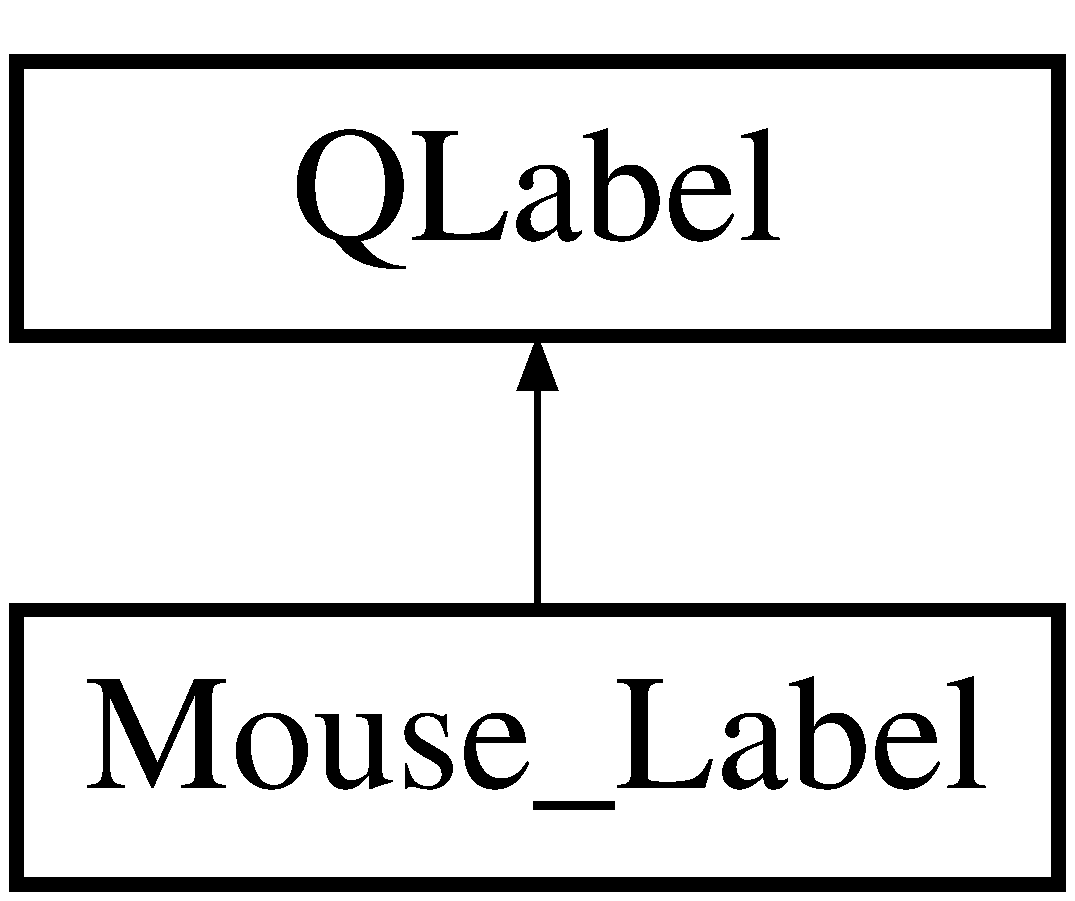
\includegraphics[height=2.000000cm]{class_mouse___label}
\end{center}
\end{figure}
\subsection*{Signals}
\begin{DoxyCompactItemize}
\item 
\hypertarget{class_mouse___label_a69e2c41ee8844e70e024b83749fd5818}{}void {\bfseries mouse\+\_\+leave} ()\label{class_mouse___label_a69e2c41ee8844e70e024b83749fd5818}

\item 
\hypertarget{class_mouse___label_a056e4e3bf3951743f674ba62d939a57f}{}void {\bfseries mouse\+\_\+enter} ()\label{class_mouse___label_a056e4e3bf3951743f674ba62d939a57f}

\item 
\hypertarget{class_mouse___label_af8de33fa7362e3d7b26b67dc2b57b717}{}void {\bfseries mouse\+\_\+move} ()\label{class_mouse___label_af8de33fa7362e3d7b26b67dc2b57b717}

\end{DoxyCompactItemize}
\subsection*{Public Member Functions}
\begin{DoxyCompactItemize}
\item 
\hypertarget{class_mouse___label_a300817fe9336be51bb68dd459b4eb686}{}{\bfseries Mouse\+\_\+\+Label} (Q\+Widget $\ast$parent=0)\label{class_mouse___label_a300817fe9336be51bb68dd459b4eb686}

\item 
\hypertarget{class_mouse___label_a267dab64326b0c5d1848eba98b0c4387}{}void {\bfseries mouse\+Move\+Event} (Q\+Mouse\+Event $\ast$)\label{class_mouse___label_a267dab64326b0c5d1848eba98b0c4387}

\item 
\hypertarget{class_mouse___label_aadd45738c71820b588a0ce659b4dba53}{}void \hyperlink{class_mouse___label_aadd45738c71820b588a0ce659b4dba53}{enter\+Event} (Q\+Event $\ast$)\label{class_mouse___label_aadd45738c71820b588a0ce659b4dba53}

\begin{DoxyCompactList}\small\item\em handles Mouse\+\_\+\+Enter\+\_\+\+Events \end{DoxyCompactList}\item 
\hypertarget{class_mouse___label_a87b74f802603230653d82a8084feab4a}{}void {\bfseries leave\+Event} (Q\+Event $\ast$)\label{class_mouse___label_a87b74f802603230653d82a8084feab4a}

\item 
\hypertarget{class_mouse___label_a25ad1b0ac37207f97dd6a478d60e4a59}{}void {\bfseries set\+Text} (const Q\+String \&)\label{class_mouse___label_a25ad1b0ac37207f97dd6a478d60e4a59}

\item 
\hypertarget{class_mouse___label_a3549cef8115331be4878c1fbd1e3c545}{}void {\bfseries clear} ()\label{class_mouse___label_a3549cef8115331be4878c1fbd1e3c545}

\item 
\hypertarget{class_mouse___label_aef5357caf49cd907267cf487f31001cd}{}void {\bfseries show} ()\label{class_mouse___label_aef5357caf49cd907267cf487f31001cd}

\item 
\hypertarget{class_mouse___label_aa28066dbc97f4f6d9901db3ebd83fe59}{}void {\bfseries clicked} ()\label{class_mouse___label_aa28066dbc97f4f6d9901db3ebd83fe59}

\item 
\hypertarget{class_mouse___label_a39b104f8fad6c48f2546a3e6e405654d}{}void {\bfseries released} ()\label{class_mouse___label_a39b104f8fad6c48f2546a3e6e405654d}

\item 
\hypertarget{class_mouse___label_a4e0732ce949e5884cb459d660964136a}{}void {\bfseries set\+Text\+\_\+\+Clicked} (Q\+String)\label{class_mouse___label_a4e0732ce949e5884cb459d660964136a}

\end{DoxyCompactItemize}


\subsection{Detailed Description}
Label subclass for the remote controller key. 

The documentation for this class was generated from the following files\+:\begin{DoxyCompactItemize}
\item 
mouse\+\_\+label.\+h\item 
mouse\+\_\+label.\+cpp\end{DoxyCompactItemize}

\hypertarget{struct_periodic_send_object}{}\section{Periodic\+Send\+Object Struct Reference}
\label{struct_periodic_send_object}\index{Periodic\+Send\+Object@{Periodic\+Send\+Object}}
\subsection*{Public Attributes}
\begin{DoxyCompactItemize}
\item 
int \hyperlink{struct_periodic_send_object_a45e7f57f2eb1c2dac99db98aeb9d87a1}{I\+D}
\begin{DoxyCompactList}\small\item\em $<$will store data that will be send periodicaly \end{DoxyCompactList}\item 
\hypertarget{struct_periodic_send_object_ace451324a4109d394e7449aa1e44ace5}{}unsigned char \hyperlink{struct_periodic_send_object_ace451324a4109d394e7449aa1e44ace5}{data} \mbox{[}14\mbox{]}\label{struct_periodic_send_object_ace451324a4109d394e7449aa1e44ace5}

\begin{DoxyCompactList}\small\item\em data that will be sent \end{DoxyCompactList}\item 
\hypertarget{struct_periodic_send_object_a0d490ee7f0807d60add8b74bb5b9149c}{}double \hyperlink{struct_periodic_send_object_a0d490ee7f0807d60add8b74bb5b9149c}{interval}\label{struct_periodic_send_object_a0d490ee7f0807d60add8b74bb5b9149c}

\begin{DoxyCompactList}\small\item\em in ms \end{DoxyCompactList}\item 
\hypertarget{struct_periodic_send_object_abc46b3afc42c71d71cf9f65f931eb81e}{}double \hyperlink{struct_periodic_send_object_abc46b3afc42c71d71cf9f65f931eb81e}{lastsent}\label{struct_periodic_send_object_abc46b3afc42c71d71cf9f65f931eb81e}

\begin{DoxyCompactList}\small\item\em in ms, set to 0 when it was never sent \end{DoxyCompactList}\item 
\hypertarget{struct_periodic_send_object_adc8d866f10d03fd22319c521062d9647}{}bool \hyperlink{struct_periodic_send_object_adc8d866f10d03fd22319c521062d9647}{active}\label{struct_periodic_send_object_adc8d866f10d03fd22319c521062d9647}

\begin{DoxyCompactList}\small\item\em data will sent if active is true \end{DoxyCompactList}\item 
\hypertarget{struct_periodic_send_object_a82892f94c820ac75f78cd60a5f292ee3}{}char \hyperlink{struct_periodic_send_object_a82892f94c820ac75f78cd60a5f292ee3}{creation}\label{struct_periodic_send_object_a82892f94c820ac75f78cd60a5f292ee3}

\begin{DoxyCompactList}\small\item\em will be set to 1 if it was created with the manual function and to 2 if it was created with the guided function \end{DoxyCompactList}\end{DoxyCompactItemize}


\subsection{Member Data Documentation}
\hypertarget{struct_periodic_send_object_a45e7f57f2eb1c2dac99db98aeb9d87a1}{}\index{Periodic\+Send\+Object@{Periodic\+Send\+Object}!I\+D@{I\+D}}
\index{I\+D@{I\+D}!Periodic\+Send\+Object@{Periodic\+Send\+Object}}
\subsubsection[{I\+D}]{\setlength{\rightskip}{0pt plus 5cm}int Periodic\+Send\+Object\+::\+I\+D}\label{struct_periodic_send_object_a45e7f57f2eb1c2dac99db98aeb9d87a1}


$<$will store data that will be send periodicaly 

I\+D for the data (not to be confused with Can I\+D) 

The documentation for this struct was generated from the following file\+:\begin{DoxyCompactItemize}
\item 
datatypes.\+h\end{DoxyCompactItemize}

\hypertarget{class_periodic_send_thread}{}\section{Periodic\+Send\+Thread Class Reference}
\label{class_periodic_send_thread}\index{Periodic\+Send\+Thread@{Periodic\+Send\+Thread}}
Inheritance diagram for Periodic\+Send\+Thread\+:\begin{figure}[H]
\begin{center}
\leavevmode
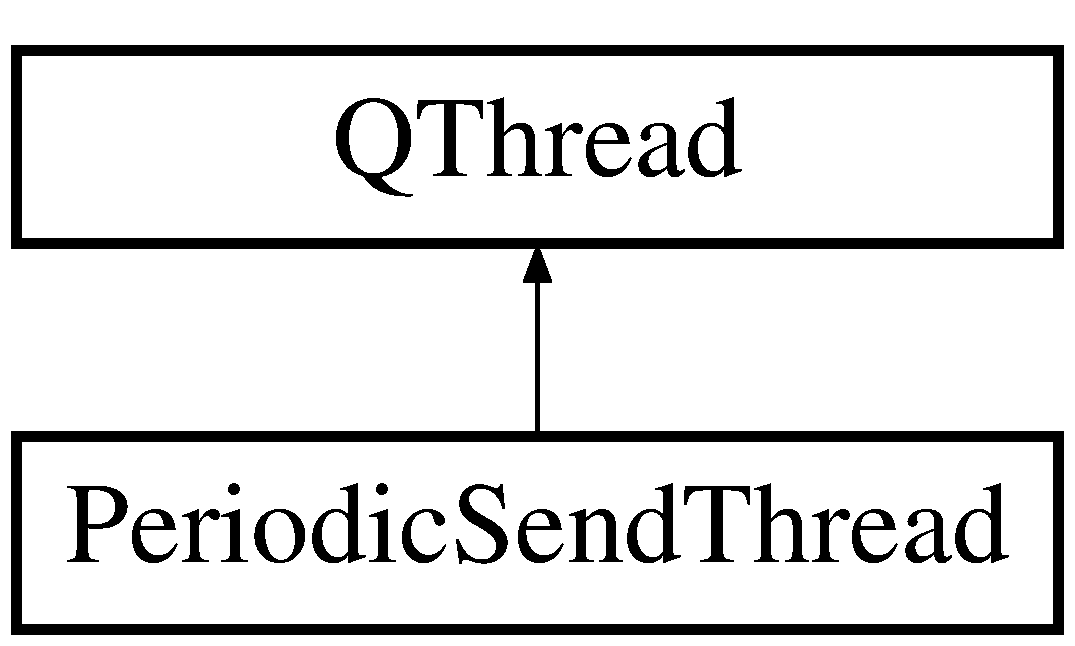
\includegraphics[height=2.000000cm]{class_periodic_send_thread}
\end{center}
\end{figure}
\subsection*{Public Member Functions}
\begin{DoxyCompactItemize}
\item 
\hypertarget{class_periodic_send_thread_aa3fa8749bbaca64c2f3719ca93a21c19}{}{\bfseries Periodic\+Send\+Thread} (Q\+Object $\ast$parent=0)\label{class_periodic_send_thread_aa3fa8749bbaca64c2f3719ca93a21c19}

\end{DoxyCompactItemize}
\subsection*{Protected Member Functions}
\begin{DoxyCompactItemize}
\item 
\hypertarget{class_periodic_send_thread_a5b6043a739a2767167d44b3bd2a184ba}{}void {\bfseries run} ()\label{class_periodic_send_thread_a5b6043a739a2767167d44b3bd2a184ba}

\end{DoxyCompactItemize}


The documentation for this class was generated from the following files\+:\begin{DoxyCompactItemize}
\item 
periodicsendthread.\+h\item 
periodicsendthread.\+cpp\end{DoxyCompactItemize}

\hypertarget{class_periodic_send_worker}{}\section{Periodic\+Send\+Worker Class Reference}
\label{class_periodic_send_worker}\index{Periodic\+Send\+Worker@{Periodic\+Send\+Worker}}


The \hyperlink{class_periodic_send_worker}{Periodic\+Send\+Worker} periodically sends messages created in the debug tab. Each message\textquotesingle{}s cycle is individually adjustable The \hyperlink{class_periodic_send_worker}{Periodic\+Send\+Worker} is created by the Main Thread to be sent afterwards to a new thread.  




{\ttfamily \#include $<$periodicsendworker.\+h$>$}

Inheritance diagram for Periodic\+Send\+Worker\+:\begin{figure}[H]
\begin{center}
\leavevmode
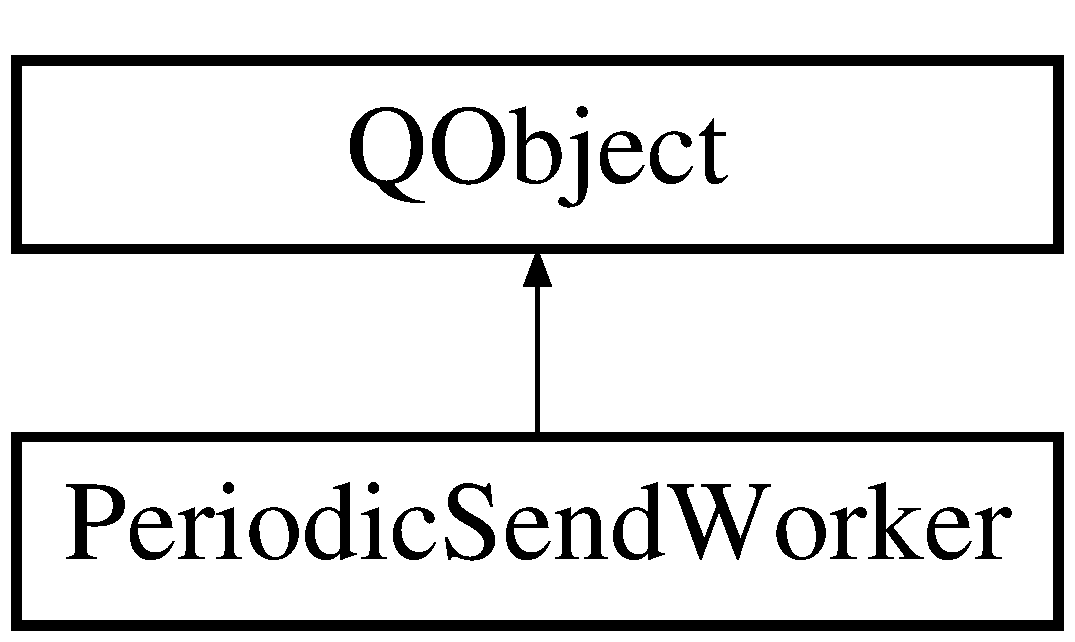
\includegraphics[height=2.000000cm]{class_periodic_send_worker}
\end{center}
\end{figure}
\subsection*{Public Slots}
\begin{DoxyCompactItemize}
\item 
\hypertarget{class_periodic_send_worker_af7d2bf362364fa72ce0321b09802b41c}{}void {\bfseries process\+\_\+start} ()\label{class_periodic_send_worker_af7d2bf362364fa72ce0321b09802b41c}

\item 
\hypertarget{class_periodic_send_worker_a3a2d60bd42d640b1d697b38334315f04}{}void {\bfseries process\+\_\+stop} ()\label{class_periodic_send_worker_a3a2d60bd42d640b1d697b38334315f04}

\end{DoxyCompactItemize}
\subsection*{Signals}
\begin{DoxyCompactItemize}
\item 
\hypertarget{class_periodic_send_worker_aaaf285a89993e59771d157fe52bf4330}{}void {\bfseries finished} (int interval)\label{class_periodic_send_worker_aaaf285a89993e59771d157fe52bf4330}

\end{DoxyCompactItemize}


\subsection{Detailed Description}
The \hyperlink{class_periodic_send_worker}{Periodic\+Send\+Worker} periodically sends messages created in the debug tab. Each message\textquotesingle{}s cycle is individually adjustable The \hyperlink{class_periodic_send_worker}{Periodic\+Send\+Worker} is created by the Main Thread to be sent afterwards to a new thread. 

The documentation for this class was generated from the following files\+:\begin{DoxyCompactItemize}
\item 
periodicsendworker.\+h\item 
periodicsendworker.\+cpp\end{DoxyCompactItemize}

\hypertarget{struct_raw_data}{}\section{Raw\+Data Struct Reference}
\label{struct_raw_data}\index{Raw\+Data@{Raw\+Data}}
\subsection*{Public Attributes}
\begin{DoxyCompactItemize}
\item 
\hypertarget{struct_raw_data_a427ce6431c739dfcdaa7d9036e327072}{}Q\+Date\+Time {\bfseries timestamp}\label{struct_raw_data_a427ce6431c739dfcdaa7d9036e327072}

\item 
\hypertarget{struct_raw_data_a77b36f8ecceafd635f6d7751210df7d1}{}unsigned char {\bfseries Raw\+Data} \mbox{[}14\mbox{]}\label{struct_raw_data_a77b36f8ecceafd635f6d7751210df7d1}

\item 
\hypertarget{struct_raw_data_ad9f56398a9e1317181663582534b0d85}{}long {\bfseries cycle}\label{struct_raw_data_ad9f56398a9e1317181663582534b0d85}

\item 
\hypertarget{struct_raw_data_ae4be078eeb0818821f793ec7ab28232a}{}int {\bfseries numberofreceiveddata}\label{struct_raw_data_ae4be078eeb0818821f793ec7ab28232a}

\end{DoxyCompactItemize}


The documentation for this struct was generated from the following file\+:\begin{DoxyCompactItemize}
\item 
datatypes.\+h\end{DoxyCompactItemize}

\hypertarget{struct_recv_buf}{}\section{Recv\+Buf Struct Reference}
\label{struct_recv_buf}\index{Recv\+Buf@{Recv\+Buf}}
\subsection*{Public Attributes}
\begin{DoxyCompactItemize}
\item 
\hypertarget{struct_recv_buf_a783259ad8d6e01768b7cec5e2e2522a0}{}Q\+Date\+Time {\bfseries timestamp}\label{struct_recv_buf_a783259ad8d6e01768b7cec5e2e2522a0}

\item 
\hypertarget{struct_recv_buf_a168ca83cef7dbeccfa3aa5a758e5d0d8}{}double {\bfseries ticks}\label{struct_recv_buf_a168ca83cef7dbeccfa3aa5a758e5d0d8}

\item 
\hypertarget{struct_recv_buf_ae3ba4d4624a4c1b2e14234293f1ad76b}{}unsigned char {\bfseries data} \mbox{[}14\mbox{]}\label{struct_recv_buf_ae3ba4d4624a4c1b2e14234293f1ad76b}

\end{DoxyCompactItemize}


The documentation for this struct was generated from the following file\+:\begin{DoxyCompactItemize}
\item 
datatypes.\+h\end{DoxyCompactItemize}

\hypertarget{class_remote_thread}{}\section{Remote\+Thread Class Reference}
\label{class_remote_thread}\index{Remote\+Thread@{Remote\+Thread}}


The \hyperlink{class_remote_thread}{Remote\+Thread} class 1\+: connection setup between Xbox\+\_\+\+Controller and mainwindow \+: Remote\+Status\+E\+X\+T=1; 2\+: if a connection to e\+C\+A\+Rus exists, a controller command will be sent to the car;.  




{\ttfamily \#include $<$remotethread.\+h$>$}

Inheritance diagram for Remote\+Thread\+:\begin{figure}[H]
\begin{center}
\leavevmode
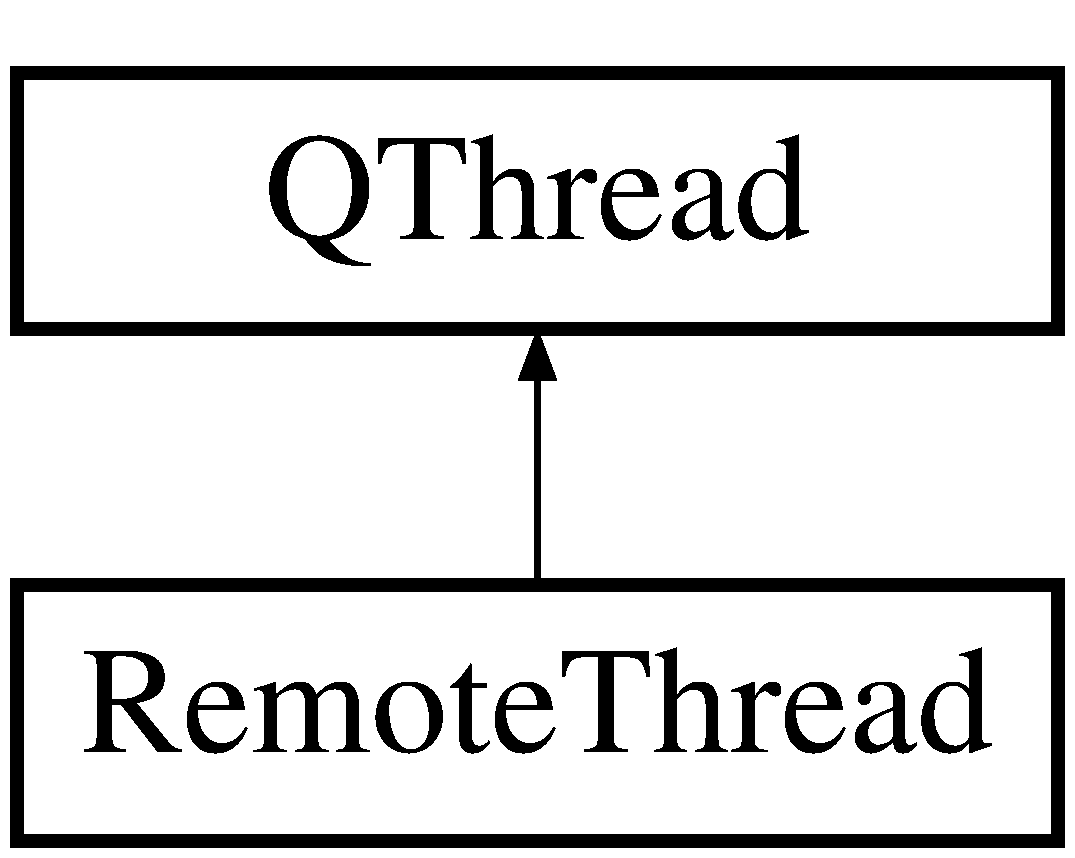
\includegraphics[height=2.000000cm]{class_remote_thread}
\end{center}
\end{figure}
\subsection*{Signals}
\begin{DoxyCompactItemize}
\item 
\hypertarget{class_remote_thread_a437bd94f9bac751befb6b7ef9dc8869f}{}void {\bfseries gear\+\_\+change} (int)\label{class_remote_thread_a437bd94f9bac751befb6b7ef9dc8869f}

\item 
\hypertarget{class_remote_thread_ab767be43aad824f123c7d0aaed84b428}{}void {\bfseries gear\+\_\+change\+\_\+\+Released} (int)\label{class_remote_thread_ab767be43aad824f123c7d0aaed84b428}

\item 
\hypertarget{class_remote_thread_acfd1278c3dea85ebbd51cd58311ca691}{}void {\bfseries x\+Button} (void)\label{class_remote_thread_acfd1278c3dea85ebbd51cd58311ca691}

\item 
\hypertarget{class_remote_thread_a004dcb4a95a7280027f766e482a1bc3d}{}void {\bfseries x\+Button\+\_\+\+Released} (void)\label{class_remote_thread_a004dcb4a95a7280027f766e482a1bc3d}

\item 
\hypertarget{class_remote_thread_a0d355904907c8f95abbde140e996f47c}{}void {\bfseries y\+Button} (void)\label{class_remote_thread_a0d355904907c8f95abbde140e996f47c}

\item 
\hypertarget{class_remote_thread_adc8c151dc217e4dd0ccdfc5673c0f851}{}void {\bfseries y\+Button\+\_\+\+Released} (void)\label{class_remote_thread_adc8c151dc217e4dd0ccdfc5673c0f851}

\item 
\hypertarget{class_remote_thread_a14dafcc79f78df3bd0dd31817ac7a322}{}void {\bfseries right\+Trigger} (void)\label{class_remote_thread_a14dafcc79f78df3bd0dd31817ac7a322}

\item 
\hypertarget{class_remote_thread_a6361b8e54d2dce24295f1c5d2d098579}{}void {\bfseries right\+Trigger\+\_\+\+Released} (void)\label{class_remote_thread_a6361b8e54d2dce24295f1c5d2d098579}

\item 
\hypertarget{class_remote_thread_abd8bcc507fcdcc4f523cfd740245be97}{}void {\bfseries left\+Trigger} (void)\label{class_remote_thread_abd8bcc507fcdcc4f523cfd740245be97}

\item 
\hypertarget{class_remote_thread_a4cb74b27bbb340d70b417ec0cbed9e3d}{}void {\bfseries left\+Trigger\+\_\+\+Released} (void)\label{class_remote_thread_a4cb74b27bbb340d70b417ec0cbed9e3d}

\item 
\hypertarget{class_remote_thread_a4e51ae0ef60c16ecf4e5c6e3ce783e6f}{}void {\bfseries start\+Button} (void)\label{class_remote_thread_a4e51ae0ef60c16ecf4e5c6e3ce783e6f}

\item 
\hypertarget{class_remote_thread_af24f62c449482783a029de8fbd78c41c}{}void {\bfseries start\+Button\+\_\+\+Released} (void)\label{class_remote_thread_af24f62c449482783a029de8fbd78c41c}

\item 
\hypertarget{class_remote_thread_aaa709e2d556a850f2a1cf2d196575435}{}void {\bfseries back\+Button} (void)\label{class_remote_thread_aaa709e2d556a850f2a1cf2d196575435}

\item 
\hypertarget{class_remote_thread_aef9ae9aa01e32f26d1a3f6d10469375a}{}void {\bfseries steering} (int)\label{class_remote_thread_aef9ae9aa01e32f26d1a3f6d10469375a}

\item 
\hypertarget{class_remote_thread_a00aba0a4f5fd8ad3d5058d53b705b175}{}void {\bfseries accelerate} (int)\label{class_remote_thread_a00aba0a4f5fd8ad3d5058d53b705b175}

\item 
\hypertarget{class_remote_thread_a54b97c7819fc4b3b8f5c0b0640b6d292}{}void {\bfseries brake} (int)\label{class_remote_thread_a54b97c7819fc4b3b8f5c0b0640b6d292}

\item 
\hypertarget{class_remote_thread_ab9e4e1c8d68eb18ce9107a89c661b2ec}{}void {\bfseries horn} (void)\label{class_remote_thread_ab9e4e1c8d68eb18ce9107a89c661b2ec}

\item 
\hypertarget{class_remote_thread_ab495f6c33d188ca3c439f1148f78e182}{}void {\bfseries horn\+\_\+\+Released} (void)\label{class_remote_thread_ab495f6c33d188ca3c439f1148f78e182}

\end{DoxyCompactItemize}
\subsection*{Public Member Functions}
\begin{DoxyCompactItemize}
\item 
\hypertarget{class_remote_thread_a1acb4cb43462156d6b9177bcb1e1dfb1}{}{\bfseries Remote\+Thread} (Q\+Object $\ast$parent=0)\label{class_remote_thread_a1acb4cb43462156d6b9177bcb1e1dfb1}

\item 
void \hyperlink{class_remote_thread_afaaf517a8ecef88feeaa477ac84da127}{run} ()
\item 
\hypertarget{class_remote_thread_ac14ef5fec27c7c93e26b59445d3eff1e}{}void {\bfseries set\+Main\+Window} (Ui\+::\+Main\+Window $\ast$w)\label{class_remote_thread_ac14ef5fec27c7c93e26b59445d3eff1e}

\item 
\hypertarget{class_remote_thread_a8da88adbd10488157ce7c634fd150f3d}{}void {\bfseries Remote\+Status\+G\+U\+I} (int)\label{class_remote_thread_a8da88adbd10488157ce7c634fd150f3d}

\item 
\hypertarget{class_remote_thread_a7eb9019a150eba70aef59e978817ac36}{}void {\bfseries Remote\+Status\+E\+X\+T} (int)\label{class_remote_thread_a7eb9019a150eba70aef59e978817ac36}

\item 
\hypertarget{class_remote_thread_a2903df0c063123c45d22d97dd55f76fa}{}void {\bfseries Remote\+Em\+Stop\+Bool} (bool)\label{class_remote_thread_a2903df0c063123c45d22d97dd55f76fa}

\item 
\hypertarget{class_remote_thread_a4dc74280db042b990cbb960b7610fa89}{}void {\bfseries Remote\+Gear\+Change} (int)\label{class_remote_thread_a4dc74280db042b990cbb960b7610fa89}

\item 
\hypertarget{class_remote_thread_af124b02a085e979b77db074994c0495b}{}void {\bfseries Remote\+Head\+Light\+Flash\+Bool} (bool)\label{class_remote_thread_af124b02a085e979b77db074994c0495b}

\item 
\hypertarget{class_remote_thread_a230a67afa07fe8ded962803751ff0acb}{}void {\bfseries Terminate} ()\label{class_remote_thread_a230a67afa07fe8ded962803751ff0acb}

\item 
\hypertarget{class_remote_thread_ac2f9c11acf7383bc97c0643ff76ac195}{}void {\bfseries toggle\+Head\+Light} ()\label{class_remote_thread_ac2f9c11acf7383bc97c0643ff76ac195}

\item 
\hypertarget{class_remote_thread_aeae85c095bf0b265d907660af3f92abd}{}void {\bfseries toggle\+Full\+Beam} ()\label{class_remote_thread_aeae85c095bf0b265d907660af3f92abd}

\item 
\hypertarget{class_remote_thread_a1de71a9c3a0a894e54b93fcb3545b3e9}{}void {\bfseries toggle\+Indicator\+Left} ()\label{class_remote_thread_a1de71a9c3a0a894e54b93fcb3545b3e9}

\item 
\hypertarget{class_remote_thread_a12da607c14e032bc0a9259891fd160c9}{}void {\bfseries toggle\+Indicator\+Right} ()\label{class_remote_thread_a12da607c14e032bc0a9259891fd160c9}

\item 
\hypertarget{class_remote_thread_aff6e6f9c8428e1e2893e52674867880f}{}void {\bfseries toggle\+Warning\+Light} ()\label{class_remote_thread_aff6e6f9c8428e1e2893e52674867880f}

\item 
\hypertarget{class_remote_thread_a23890ade40fb63ad7d2a8d837bfbad13}{}void {\bfseries turn\+Off\+Head\+Light} ()\label{class_remote_thread_a23890ade40fb63ad7d2a8d837bfbad13}

\item 
\hypertarget{class_remote_thread_a2c5f6d0d0dc96d020553366d90601909}{}void {\bfseries turn\+Off\+Full\+Beam} ()\label{class_remote_thread_a2c5f6d0d0dc96d020553366d90601909}

\item 
\hypertarget{class_remote_thread_a610ccdb470eba1e3343508ac0c9e77f4}{}void {\bfseries turn\+Off\+Indicator\+Left} ()\label{class_remote_thread_a610ccdb470eba1e3343508ac0c9e77f4}

\item 
\hypertarget{class_remote_thread_a4cb09cd54f412b5f75c03f1aabcea1c4}{}void {\bfseries turn\+Off\+Indicator\+Right} ()\label{class_remote_thread_a4cb09cd54f412b5f75c03f1aabcea1c4}

\item 
\hypertarget{class_remote_thread_a1fd04f4c01e8eff1f9026f5527b8985d}{}void {\bfseries turn\+Off\+Warning\+Light} ()\label{class_remote_thread_a1fd04f4c01e8eff1f9026f5527b8985d}

\item 
\hypertarget{class_remote_thread_a24a11ba01cfd56b677d8ab86c68a1a03}{}int {\bfseries Remote\+Status\+G\+U\+I} ()\label{class_remote_thread_a24a11ba01cfd56b677d8ab86c68a1a03}

\item 
\hypertarget{class_remote_thread_af3983983a7ffc901ad46d8cab5165be2}{}int {\bfseries Remote\+Status\+E\+X\+T} ()\label{class_remote_thread_af3983983a7ffc901ad46d8cab5165be2}

\item 
\hypertarget{class_remote_thread_ad3ea0c38f8964e13a54029ff3b57f9be}{}bool {\bfseries Remote\+Em\+Stop\+Bool} ()\label{class_remote_thread_ad3ea0c38f8964e13a54029ff3b57f9be}

\item 
\hypertarget{class_remote_thread_a8e38bf53fe6999bd9c9422dba444b488}{}int {\bfseries Remote\+Gear\+Change} ()\label{class_remote_thread_a8e38bf53fe6999bd9c9422dba444b488}

\item 
\hypertarget{class_remote_thread_abe6ace2c5a7ea3e07442356410193176}{}bool {\bfseries Remote\+Head\+Light\+Flash\+Bool} ()\label{class_remote_thread_abe6ace2c5a7ea3e07442356410193176}

\item 
\hypertarget{class_remote_thread_a23d858237047288708045248766026c2}{}bool {\bfseries Terminated} ()\label{class_remote_thread_a23d858237047288708045248766026c2}

\item 
\hypertarget{class_remote_thread_affbec79b15b16bb2fa90ec2478e2e011}{}bool {\bfseries head\+Light\+Is\+On} ()\label{class_remote_thread_affbec79b15b16bb2fa90ec2478e2e011}

\item 
\hypertarget{class_remote_thread_abc8331efb2c5b8db1a2ad4f16d128488}{}bool {\bfseries full\+Beam\+Is\+On} ()\label{class_remote_thread_abc8331efb2c5b8db1a2ad4f16d128488}

\item 
\hypertarget{class_remote_thread_a07174c7e23b2a77077d5b539bb83cb9a}{}bool {\bfseries indicator\+Left\+Is\+On} ()\label{class_remote_thread_a07174c7e23b2a77077d5b539bb83cb9a}

\item 
\hypertarget{class_remote_thread_ae3cd54f0f87da2278dacc7f0222b8c47}{}bool {\bfseries indicator\+Right\+Is\+On} ()\label{class_remote_thread_ae3cd54f0f87da2278dacc7f0222b8c47}

\item 
\hypertarget{class_remote_thread_a2c2d3788a456b99d633ba1dd14e308e5}{}bool {\bfseries warning\+Light\+Is\+On} ()\label{class_remote_thread_a2c2d3788a456b99d633ba1dd14e308e5}

\item 
\hypertarget{class_remote_thread_ae376c77e15ff8adb7b60028ad92547bb}{}void {\bfseries init\+\_\+\+Remote\+Status\+G\+U\+I} (int $\ast$)\label{class_remote_thread_ae376c77e15ff8adb7b60028ad92547bb}

\item 
\hypertarget{class_remote_thread_ad69aba3296b67a50b8dff3c22f7e89a0}{}void {\bfseries init\+\_\+\+Remote\+Status\+E\+X\+T} (int $\ast$)\label{class_remote_thread_ad69aba3296b67a50b8dff3c22f7e89a0}

\item 
\hypertarget{class_remote_thread_a659f51b16da9cdb8caf52f0c885d2be6}{}void {\bfseries init\+\_\+head\+Light\+Is\+On} (bool $\ast$)\label{class_remote_thread_a659f51b16da9cdb8caf52f0c885d2be6}

\item 
\hypertarget{class_remote_thread_a6d1ea3bd7e4a7ff4c2e0665699bae8f9}{}void {\bfseries init\+\_\+full\+Beam\+Is\+On} (bool $\ast$)\label{class_remote_thread_a6d1ea3bd7e4a7ff4c2e0665699bae8f9}

\item 
\hypertarget{class_remote_thread_a3b2cadf9a68f30c60520ec7b4ef2dcce}{}void {\bfseries init\+\_\+indicator\+Left\+Is\+On} (bool $\ast$)\label{class_remote_thread_a3b2cadf9a68f30c60520ec7b4ef2dcce}

\item 
\hypertarget{class_remote_thread_a254eceb6b4f4089e7b102abdb420af6d}{}void {\bfseries init\+\_\+indicator\+Right\+Is\+On} (bool $\ast$)\label{class_remote_thread_a254eceb6b4f4089e7b102abdb420af6d}

\item 
\hypertarget{class_remote_thread_ac925727df6675d74636db3ee90fb2717}{}void {\bfseries init\+\_\+warning\+Light\+Is\+On} (bool $\ast$)\label{class_remote_thread_ac925727df6675d74636db3ee90fb2717}

\item 
\hypertarget{class_remote_thread_af15651120a1ed1a43d54fe0b562a68c9}{}void {\bfseries init\+\_\+\+Remote\+Em\+Stop\+Bool} (bool $\ast$)\label{class_remote_thread_af15651120a1ed1a43d54fe0b562a68c9}

\item 
\hypertarget{class_remote_thread_afbfe2a847389c2633f3c1f5b3ef282dc}{}void {\bfseries init\+\_\+\+Remote\+Gear\+Change} (int $\ast$)\label{class_remote_thread_afbfe2a847389c2633f3c1f5b3ef282dc}

\item 
\hypertarget{class_remote_thread_a996adb972df55c57ef020e199a2edc80}{}void {\bfseries init\+\_\+\+Remote\+Head\+Light\+Flash\+Bool} (bool $\ast$)\label{class_remote_thread_a996adb972df55c57ef020e199a2edc80}

\item 
\hypertarget{class_remote_thread_ae5f3eaba7830d9bdf5ca2f05c212b160}{}void {\bfseries init\+\_\+\+Terminated} (bool $\ast$)\label{class_remote_thread_ae5f3eaba7830d9bdf5ca2f05c212b160}

\item 
\hypertarget{class_remote_thread_aca0c6a9df3fb70119fb2bd4a7e40f8af}{}void {\bfseries init\+\_\+\+Remote\+Gear} (int $\ast$)\label{class_remote_thread_aca0c6a9df3fb70119fb2bd4a7e40f8af}

\item 
\hypertarget{class_remote_thread_ab926c7f3a9ba29a1df52993a1747c128}{}void {\bfseries init\+\_\+\+Remote\+Setting\+\_\+1} (int $\ast$)\label{class_remote_thread_ab926c7f3a9ba29a1df52993a1747c128}

\item 
\hypertarget{class_remote_thread_ad0362858a88dc58310be1171d22239c0}{}void {\bfseries init\+\_\+\+Remote\+Setting\+\_\+2} (int $\ast$)\label{class_remote_thread_ad0362858a88dc58310be1171d22239c0}

\item 
\hypertarget{class_remote_thread_a37156a23aea69e77fd86cf97599afd08}{}void {\bfseries init\+\_\+\+Remote\+Setting\+\_\+3} (int $\ast$)\label{class_remote_thread_a37156a23aea69e77fd86cf97599afd08}

\end{DoxyCompactItemize}
\subsection*{Public Attributes}
\begin{DoxyCompactItemize}
\item 
\hypertarget{class_remote_thread_a668f3195a6b2fd7f7881398ad8c0537f}{}float {\bfseries Max\+Speed}\label{class_remote_thread_a668f3195a6b2fd7f7881398ad8c0537f}

\end{DoxyCompactItemize}


\subsection{Detailed Description}
The \hyperlink{class_remote_thread}{Remote\+Thread} class 1\+: connection setup between Xbox\+\_\+\+Controller and mainwindow \+: Remote\+Status\+E\+X\+T=1; 2\+: if a connection to e\+C\+A\+Rus exists, a controller command will be sent to the car;. 

\subsection{Member Function Documentation}
\hypertarget{class_remote_thread_afaaf517a8ecef88feeaa477ac84da127}{}\index{Remote\+Thread@{Remote\+Thread}!run@{run}}
\index{run@{run}!Remote\+Thread@{Remote\+Thread}}
\subsubsection[{run()}]{\setlength{\rightskip}{0pt plus 5cm}void Remote\+Thread\+::run (
\begin{DoxyParamCaption}
{}
\end{DoxyParamCaption}
)}\label{class_remote_thread_afaaf517a8ecef88feeaa477ac84da127}
called when the value of the bright trigger changes 
\begin{DoxyParams}{Parameters}
{\em value} & position of the slider\\
\hline
\end{DoxyParams}
langert text.( it linearizes the characteristic curve of the accelerator )

The documentation for this class was generated from the following files\+:\begin{DoxyCompactItemize}
\item 
remotethread.\+h\item 
remotethread.\+cpp\end{DoxyCompactItemize}

\hypertarget{class_special___label}{}\section{Special\+\_\+\+Label Class Reference}
\label{class_special___label}\index{Special\+\_\+\+Label@{Special\+\_\+\+Label}}


The \hyperlink{class_special___label}{Special\+\_\+\+Label} class is able to handle Mouse Events by emitting individual signals for each mouse event.  




{\ttfamily \#include $<$special\+\_\+label.\+h$>$}

Inheritance diagram for Special\+\_\+\+Label\+:\begin{figure}[H]
\begin{center}
\leavevmode
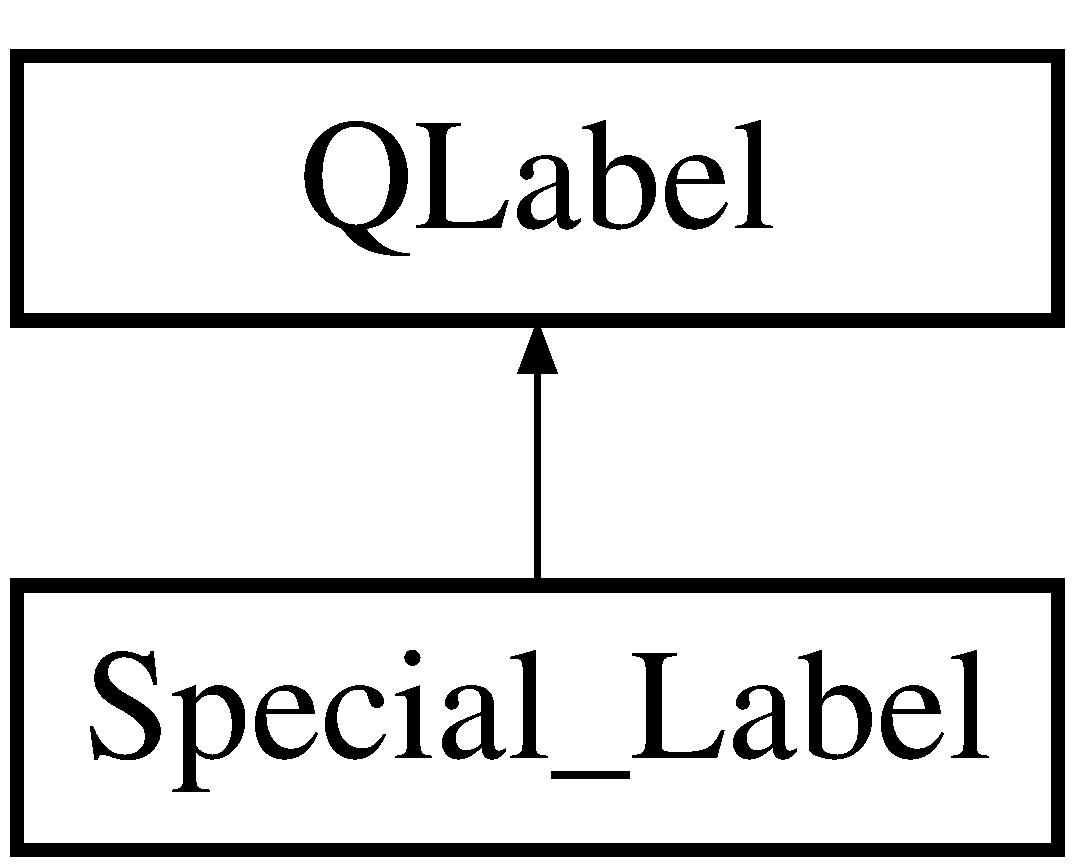
\includegraphics[height=2.000000cm]{class_special___label}
\end{center}
\end{figure}
\subsection*{Public Slots}
\begin{DoxyCompactItemize}
\item 
\hypertarget{class_special___label_a8d6f52208b95cf7479801d6a897ab381}{}void {\bfseries mouse\+Move\+Event} (Q\+Mouse\+Event $\ast$)\label{class_special___label_a8d6f52208b95cf7479801d6a897ab381}

\end{DoxyCompactItemize}
\subsection*{Signals}
\begin{DoxyCompactItemize}
\item 
\hypertarget{class_special___label_ad9904bc86cee59bb283a6e9188f0f669}{}void {\bfseries mouse\+\_\+leave} ()\label{class_special___label_ad9904bc86cee59bb283a6e9188f0f669}

\item 
\hypertarget{class_special___label_a063b6e6dad3dd00e999460445d3d9d52}{}void {\bfseries mouse\+\_\+enter} ()\label{class_special___label_a063b6e6dad3dd00e999460445d3d9d52}

\item 
\hypertarget{class_special___label_a0b40214ec4cf873b827a159ff769b6f1}{}void {\bfseries mouse\+\_\+move} ()\label{class_special___label_a0b40214ec4cf873b827a159ff769b6f1}

\item 
\hypertarget{class_special___label_aade99d0d26d7bf83c8b3a27ab9b89247}{}void {\bfseries mouse\+\_\+click} ()\label{class_special___label_aade99d0d26d7bf83c8b3a27ab9b89247}

\item 
\hypertarget{class_special___label_a3d7ff26e67dbc15114af50f904910fd7}{}void {\bfseries mouse\+\_\+release} ()\label{class_special___label_a3d7ff26e67dbc15114af50f904910fd7}

\end{DoxyCompactItemize}
\subsection*{Public Member Functions}
\begin{DoxyCompactItemize}
\item 
\hypertarget{class_special___label_a0521e7c5122e0827ab4007007d7e0c65}{}{\bfseries Special\+\_\+\+Label} (Q\+Widget $\ast$parent=0)\label{class_special___label_a0521e7c5122e0827ab4007007d7e0c65}

\item 
\hypertarget{class_special___label_a40c6006c6e0b1948104d4cbbc44d3fdc}{}void {\bfseries enter\+Event} (Q\+Event $\ast$)\label{class_special___label_a40c6006c6e0b1948104d4cbbc44d3fdc}

\item 
\hypertarget{class_special___label_a12e3db53d0413b2b664c0f7fd2cfa153}{}void {\bfseries leave\+Event} (Q\+Event $\ast$)\label{class_special___label_a12e3db53d0413b2b664c0f7fd2cfa153}

\item 
\hypertarget{class_special___label_a69b1cf24e1719c0a555e55d43dee1c31}{}void {\bfseries clicked} ()\label{class_special___label_a69b1cf24e1719c0a555e55d43dee1c31}

\item 
\hypertarget{class_special___label_a1143161eb572b45e556c7c794d1d7121}{}void {\bfseries released} ()\label{class_special___label_a1143161eb572b45e556c7c794d1d7121}

\item 
\hypertarget{class_special___label_a5ae3fe5084663c4541faa7466a23fefa}{}void {\bfseries mouse\+Press\+Event} (Q\+Mouse\+Event $\ast$ev)\label{class_special___label_a5ae3fe5084663c4541faa7466a23fefa}

\item 
\hypertarget{class_special___label_a46cb081e9b71bf02a9180541936af411}{}void {\bfseries mouse\+Release\+Event} (Q\+Mouse\+Event $\ast$ev)\label{class_special___label_a46cb081e9b71bf02a9180541936af411}

\end{DoxyCompactItemize}


\subsection{Detailed Description}
The \hyperlink{class_special___label}{Special\+\_\+\+Label} class is able to handle Mouse Events by emitting individual signals for each mouse event. 

The documentation for this class was generated from the following files\+:\begin{DoxyCompactItemize}
\item 
special\+\_\+label.\+h\item 
special\+\_\+label.\+cpp\end{DoxyCompactItemize}

\hypertarget{class_u_d_p_thread}{}\section{U\+D\+P\+Thread Class Reference}
\label{class_u_d_p_thread}\index{U\+D\+P\+Thread@{U\+D\+P\+Thread}}


The \hyperlink{class_u_d_p_thread}{U\+D\+P\+Thread} class is able to send and receive messages Messages, which are resided in the Udp\+Socket, will be enqueued to the Recv\+Buf-\/\+Queue Rec\+Queue Messages, which are supposed to be send by the software, will be resided in the Udp\+Socket.  




{\ttfamily \#include $<$udpthread.\+h$>$}

Inheritance diagram for U\+D\+P\+Thread\+:\begin{figure}[H]
\begin{center}
\leavevmode
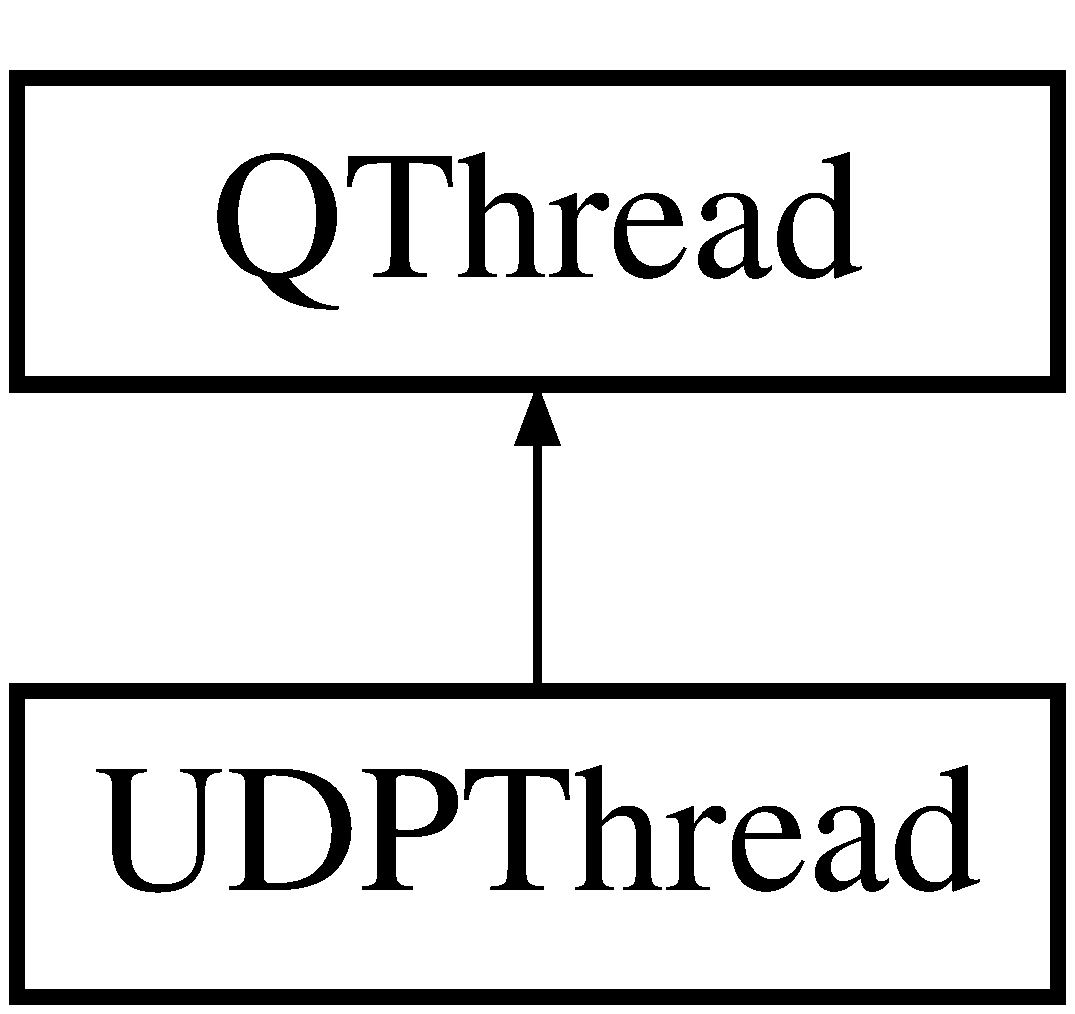
\includegraphics[height=2.000000cm]{class_u_d_p_thread}
\end{center}
\end{figure}
\subsection*{Signals}
\begin{DoxyCompactItemize}
\item 
\hypertarget{class_u_d_p_thread_a69d3f7b11b8741a043c0e0e8c96896b3}{}void {\bfseries receive\+\_\+datagram} (Q\+Byte\+Array)\label{class_u_d_p_thread_a69d3f7b11b8741a043c0e0e8c96896b3}

\end{DoxyCompactItemize}
\subsection*{Public Member Functions}
\begin{DoxyCompactItemize}
\item 
\hypertarget{class_u_d_p_thread_a90ab3e13bf9c4df446c2126ab76b0ef5}{}{\bfseries U\+D\+P\+Thread} (Q\+Object $\ast$parent=0)\label{class_u_d_p_thread_a90ab3e13bf9c4df446c2126ab76b0ef5}

\item 
\hypertarget{class_u_d_p_thread_a588f976d998e8da61fe4887bb2297e24}{}void {\bfseries U\+Iswitchtoconnect} ()\label{class_u_d_p_thread_a588f976d998e8da61fe4887bb2297e24}

\item 
\hypertarget{class_u_d_p_thread_a4c296054132eea751c34103e66fbcac4}{}void {\bfseries Setup\+Thread} (Q\+String, Q\+String)\label{class_u_d_p_thread_a4c296054132eea751c34103e66fbcac4}

\item 
\hypertarget{class_u_d_p_thread_a456f8ce6d9f1e29f4d7797ffc799fae4}{}void {\bfseries Finish\+Thread} ()\label{class_u_d_p_thread_a456f8ce6d9f1e29f4d7797ffc799fae4}

\end{DoxyCompactItemize}
\subsection*{Protected Member Functions}
\begin{DoxyCompactItemize}
\item 
\hypertarget{class_u_d_p_thread_a1ef491338c2f7b358968505b82a73a87}{}void \hyperlink{class_u_d_p_thread_a1ef491338c2f7b358968505b82a73a87}{run} ()\label{class_u_d_p_thread_a1ef491338c2f7b358968505b82a73a87}

\begin{DoxyCompactList}\small\item\em run Binds to the udp socket S\+E\+N\+D\+I\+N\+G\+: The method dequeues the messages, which are to be sent, from the message queue Send\+Data and writes the \hyperlink{struct_raw_data}{Raw\+Data} to the udp socket R\+E\+C\+E\+I\+V\+I\+N\+G\+: \hyperlink{class_u_d_p_thread_a1ef491338c2f7b358968505b82a73a87}{run()} converts the datagrams of the udp socket to \hyperlink{struct_recv_buf}{Recv\+Buf} and pushes the data to the queue Rec\+Queue \end{DoxyCompactList}\end{DoxyCompactItemize}


\subsection{Detailed Description}
The \hyperlink{class_u_d_p_thread}{U\+D\+P\+Thread} class is able to send and receive messages Messages, which are resided in the Udp\+Socket, will be enqueued to the Recv\+Buf-\/\+Queue Rec\+Queue Messages, which are supposed to be send by the software, will be resided in the Udp\+Socket. 

The documentation for this class was generated from the following files\+:\begin{DoxyCompactItemize}
\item 
udpthread.\+h\item 
udpthread.\+cpp\end{DoxyCompactItemize}

%--- End generated contents ---

% Index
\backmatter
\newpage
\phantomsection
\clearemptydoublepage
\addcontentsline{toc}{chapter}{Index}
\printindex

\end{document}
